\section{Signal Independent Limits}
%   \label{sec:signalIndependentLimits}% uncomment if label used. 
    \subsection{Untagged Resonances: Model-independent Gaussian Limits}
%       \label{subsec:UntaggedResonancesGaussianLimits} % uncomment if label used. 
        It is important to set limits on the cross-section of model-independent signals both to expand the analysis' search to include sensitivity to new signals that may be detectable with this analysis but which are not currently theoretically motivated, and to have a reasonable way to evaluate and compare the strength of different analyses without biasing this comparison by the choice of model (as all analyses have specific models they are more or less sensitive to).

        To produce model-independent limits in this analysis which is resonance based, it is required to have a 'model-independent' resonance signal. The analysis is sensitive to the resonance shape, which is strongly influenced by specific models. This is in general a good feature of the analysis which allows the ability to distinguish different signal models, however this results in any model-independent limits being set being implicitly influenced by the shape of the resonance that is chosen to produce these model-independent limits. To ensure these limits are as model-independent as possible then, it is important to choose a resonance shape that is similar to the 'average' signal. A proxy for this was chosen to be a Gaussian resonance with varying widths, as a dominant contribution to the shape of any realistic signal without very specific model-dependent assumptions is the jet resolution which produces an approximately gaussian resonance after reconstruction, and hence a gaussian resonance should approximately describe any realistic resonance.

        The untagged $y^{*} < 0.8$, 1-$g$ tagged $y^{*} < 0.6$ \& 2-$g$ tagged $y^{*} < 0.8$ model-independent Gaussian limits are shown in Figures \ref{fig:SignalIndependentGaussianLimits_UntaggedYStar0p8}, \ref{fig:SignalIndependentGaussianLimits_1gYStar0p6} \& \ref{fig:SignalIndependentGaussianLimits_2gYStar0p8} respectively, for Gaussians with width equal to 0,3,5,7,10 \& 15\% of their peak position, without systematics included. There are small issues particularly with fit convergence in the higher width resonances which is currently being investigated.

        \begin{figure}[!htb]
            \subfigure[0\% Width Gaussian Limits]{ 
%                \label{fig:SignalIndependentGaussianLimits_SubWidth0} % uncomment if label used. 
                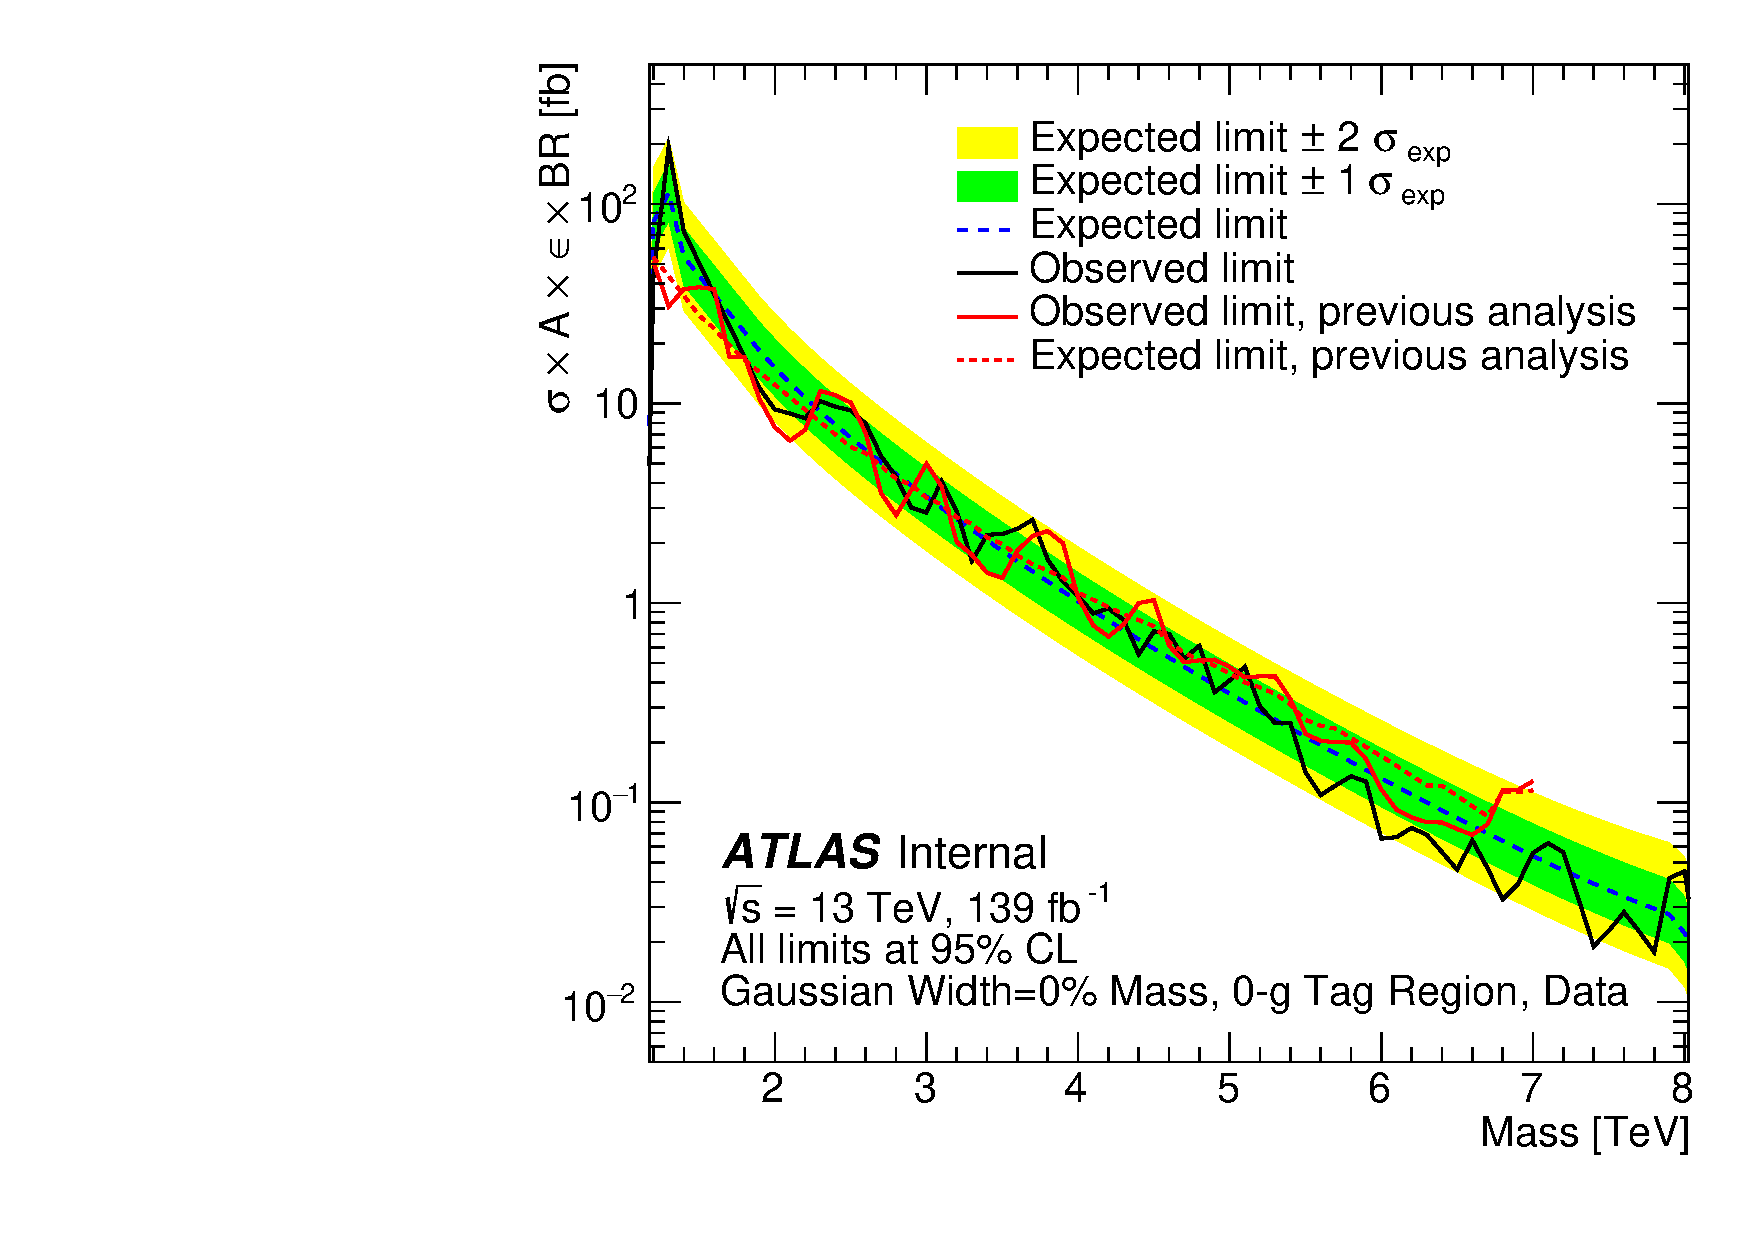
\includegraphics[width=0.3\textwidth]{figures/app-SignalIndependentLimits/Gauss_Limits_yStar0p8_Tag0_WidthPercent0_1200to8000_sigma.pdf}
            }
            \subfigure[3\% Width Gaussian Limits]{ 
%                \label{fig:SignalIndependentGaussianLimits_SubWidth3} % uncomment if label used. 
                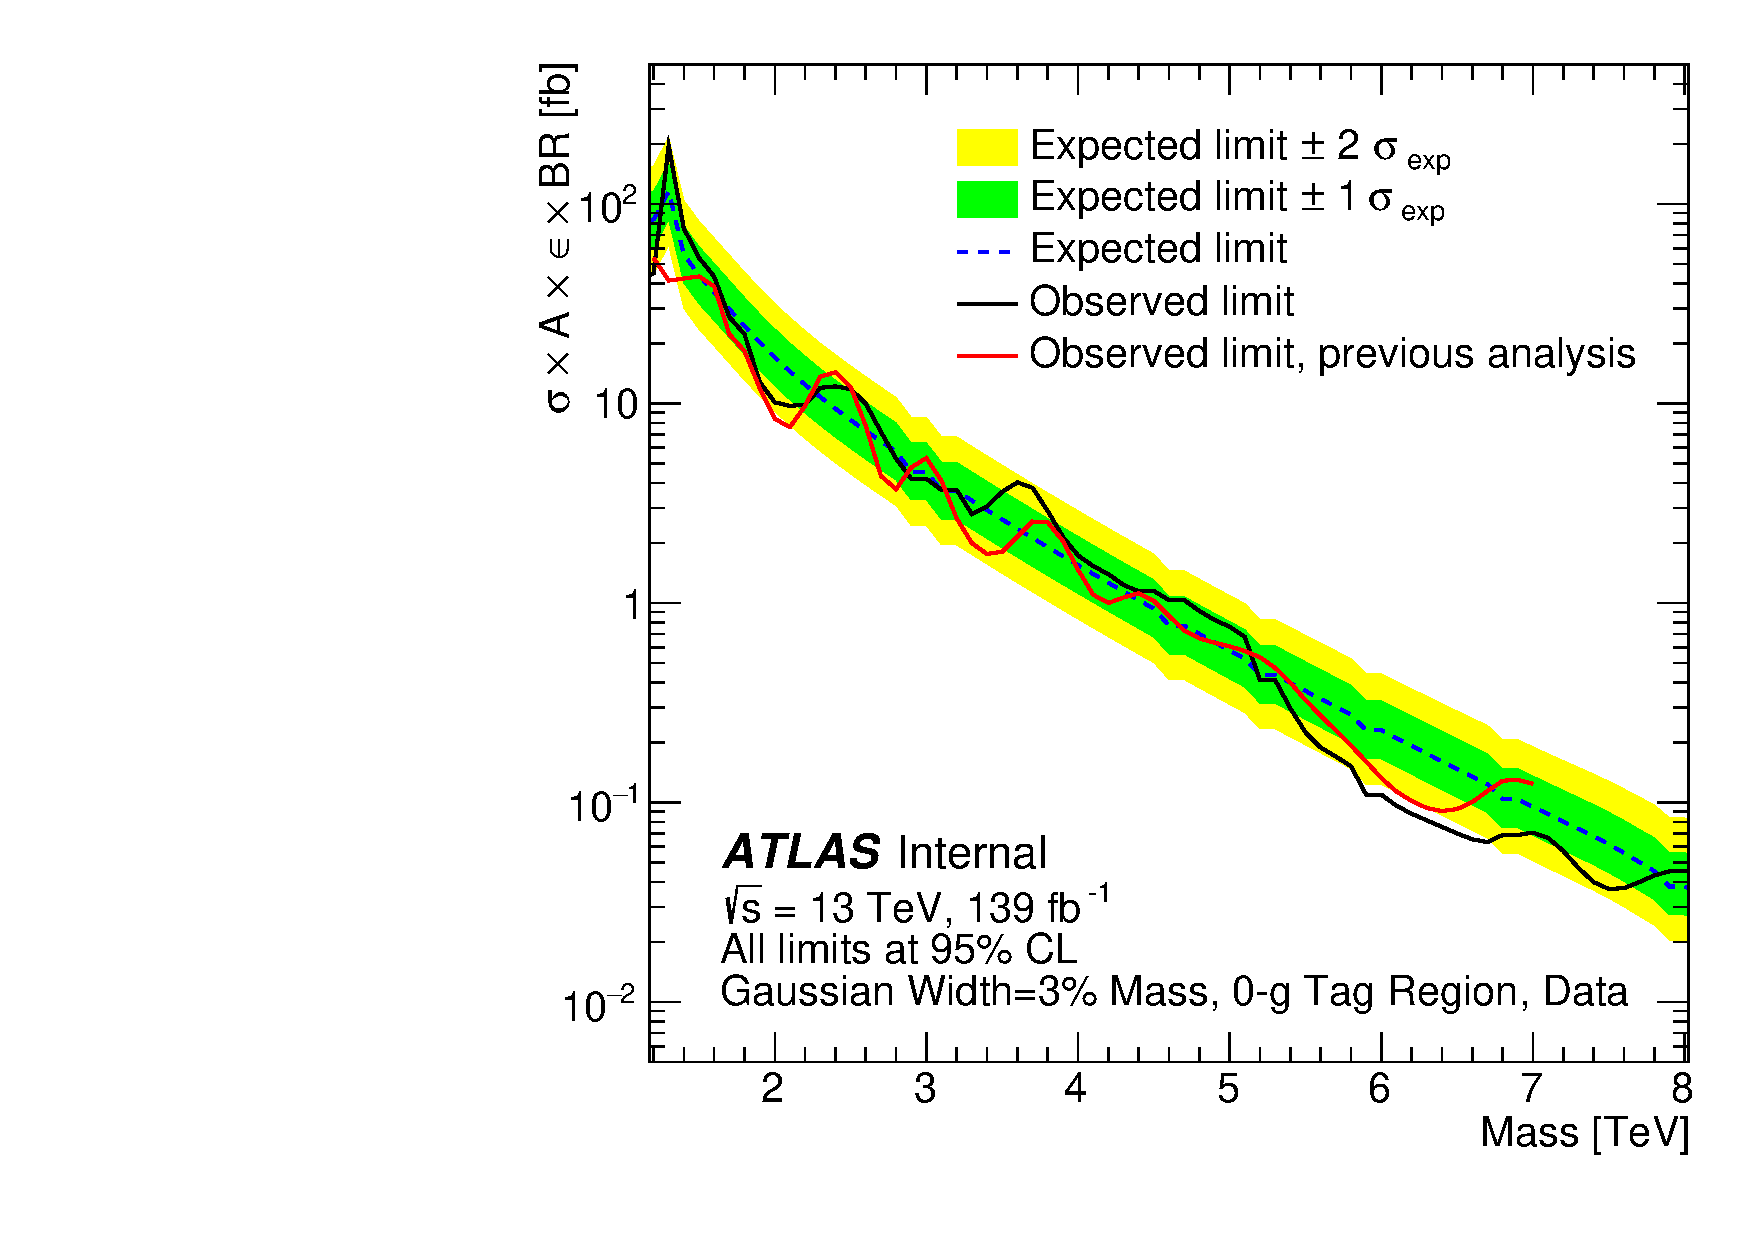
\includegraphics[width=0.3\textwidth]{figures/app-SignalIndependentLimits/Gauss_Limits_yStar0p8_Tag0_WidthPercent3_1200to8000_sigma.pdf}
            }
            \subfigure[5\% Width Gaussian Limits]{ 
%                \label{fig:SignalIndependentGaussianLimits_SubWidth5} % uncomment if label used. 
                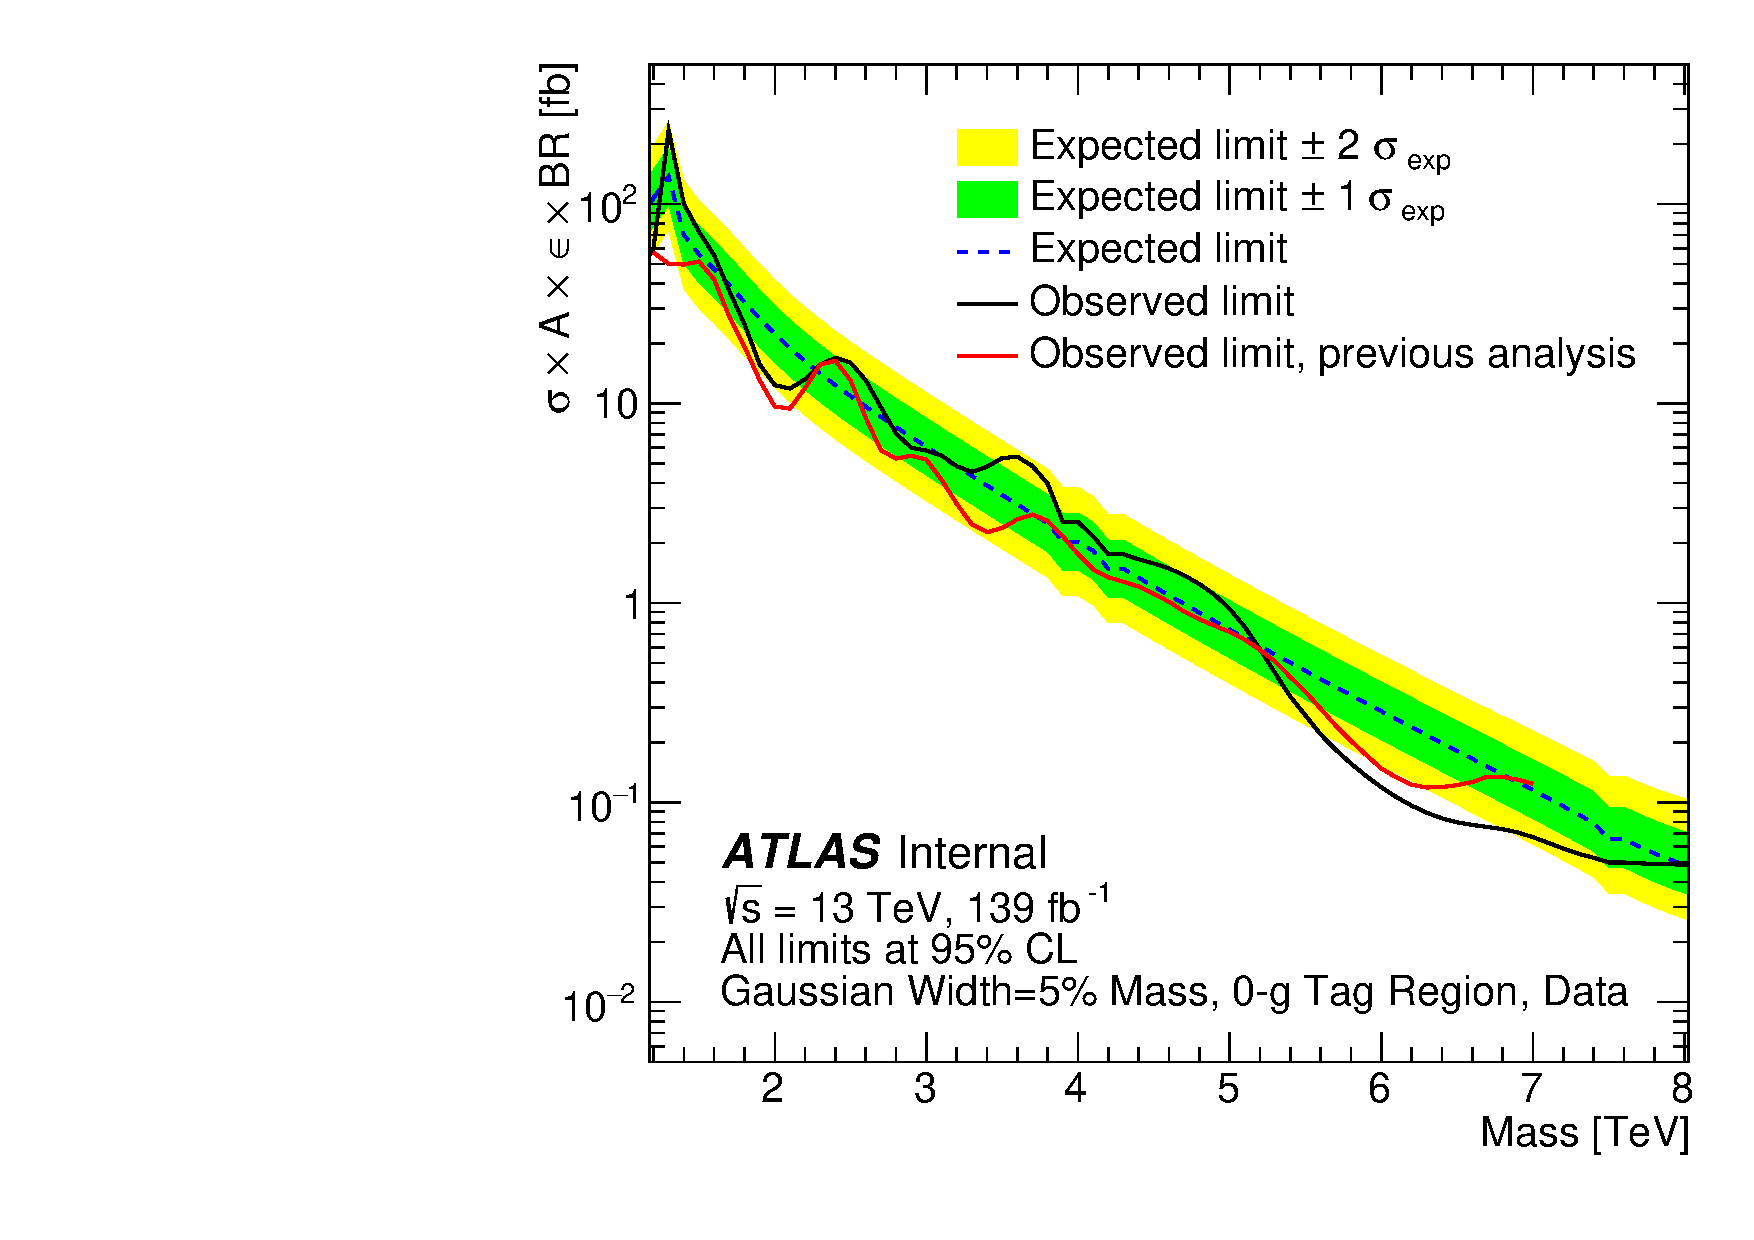
\includegraphics[width=0.3\textwidth]{figures/app-SignalIndependentLimits/Gauss_Limits_yStar0p8_Tag0_WidthPercent5_1200to8000_sigma.pdf}
            }
            \subfigure[7\% Width Gaussian Limits]{ 
%                \label{fig:SignalIndependentGaussianLimits_SubWidth7} % uncomment if label used. 
                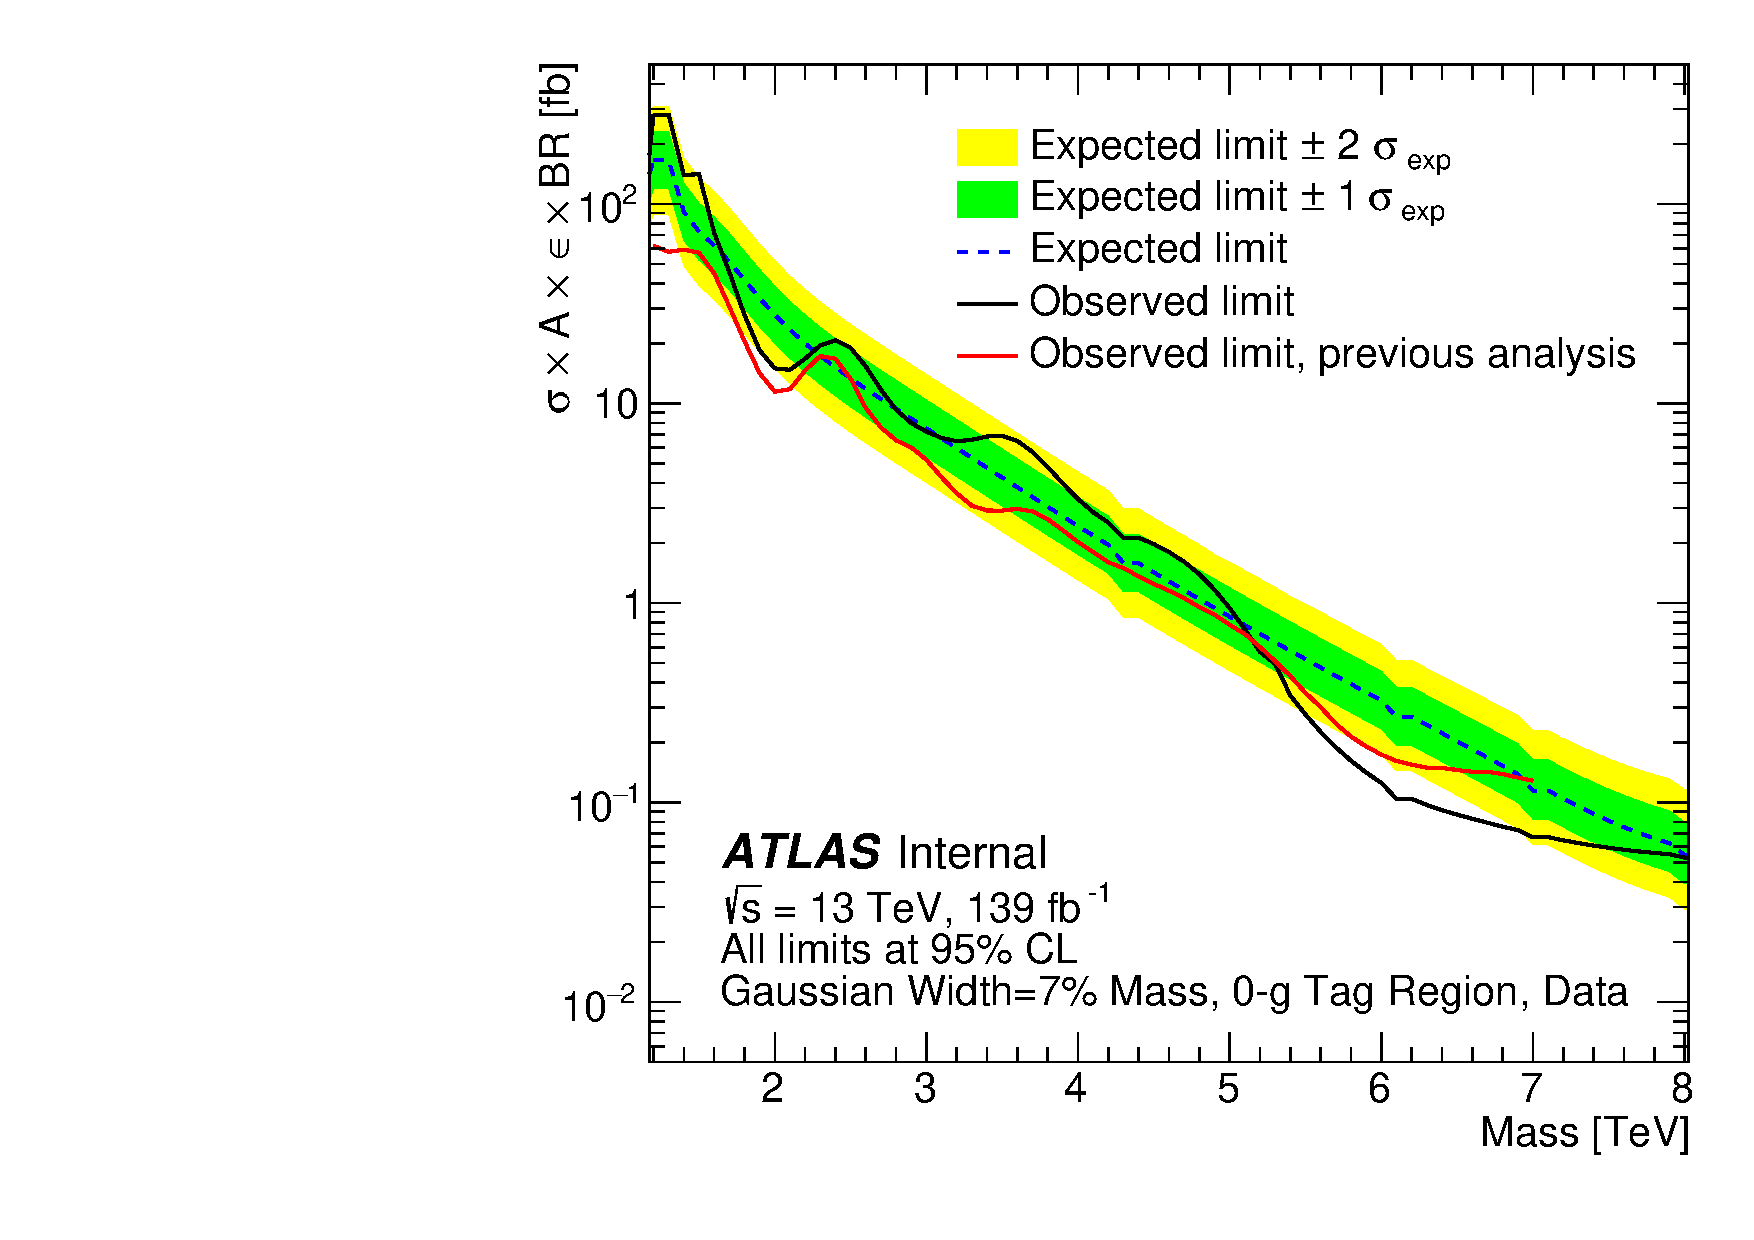
\includegraphics[width=0.3\textwidth]{figures/app-SignalIndependentLimits/Gauss_Limits_yStar0p8_Tag0_WidthPercent7_1200to8000_sigma.pdf}
            }
            \subfigure[10\% Width Gaussian Limits]{ 
%                \label{fig:SignalIndependentGaussianLimits_SubWidth10} % uncomment if label used. 
                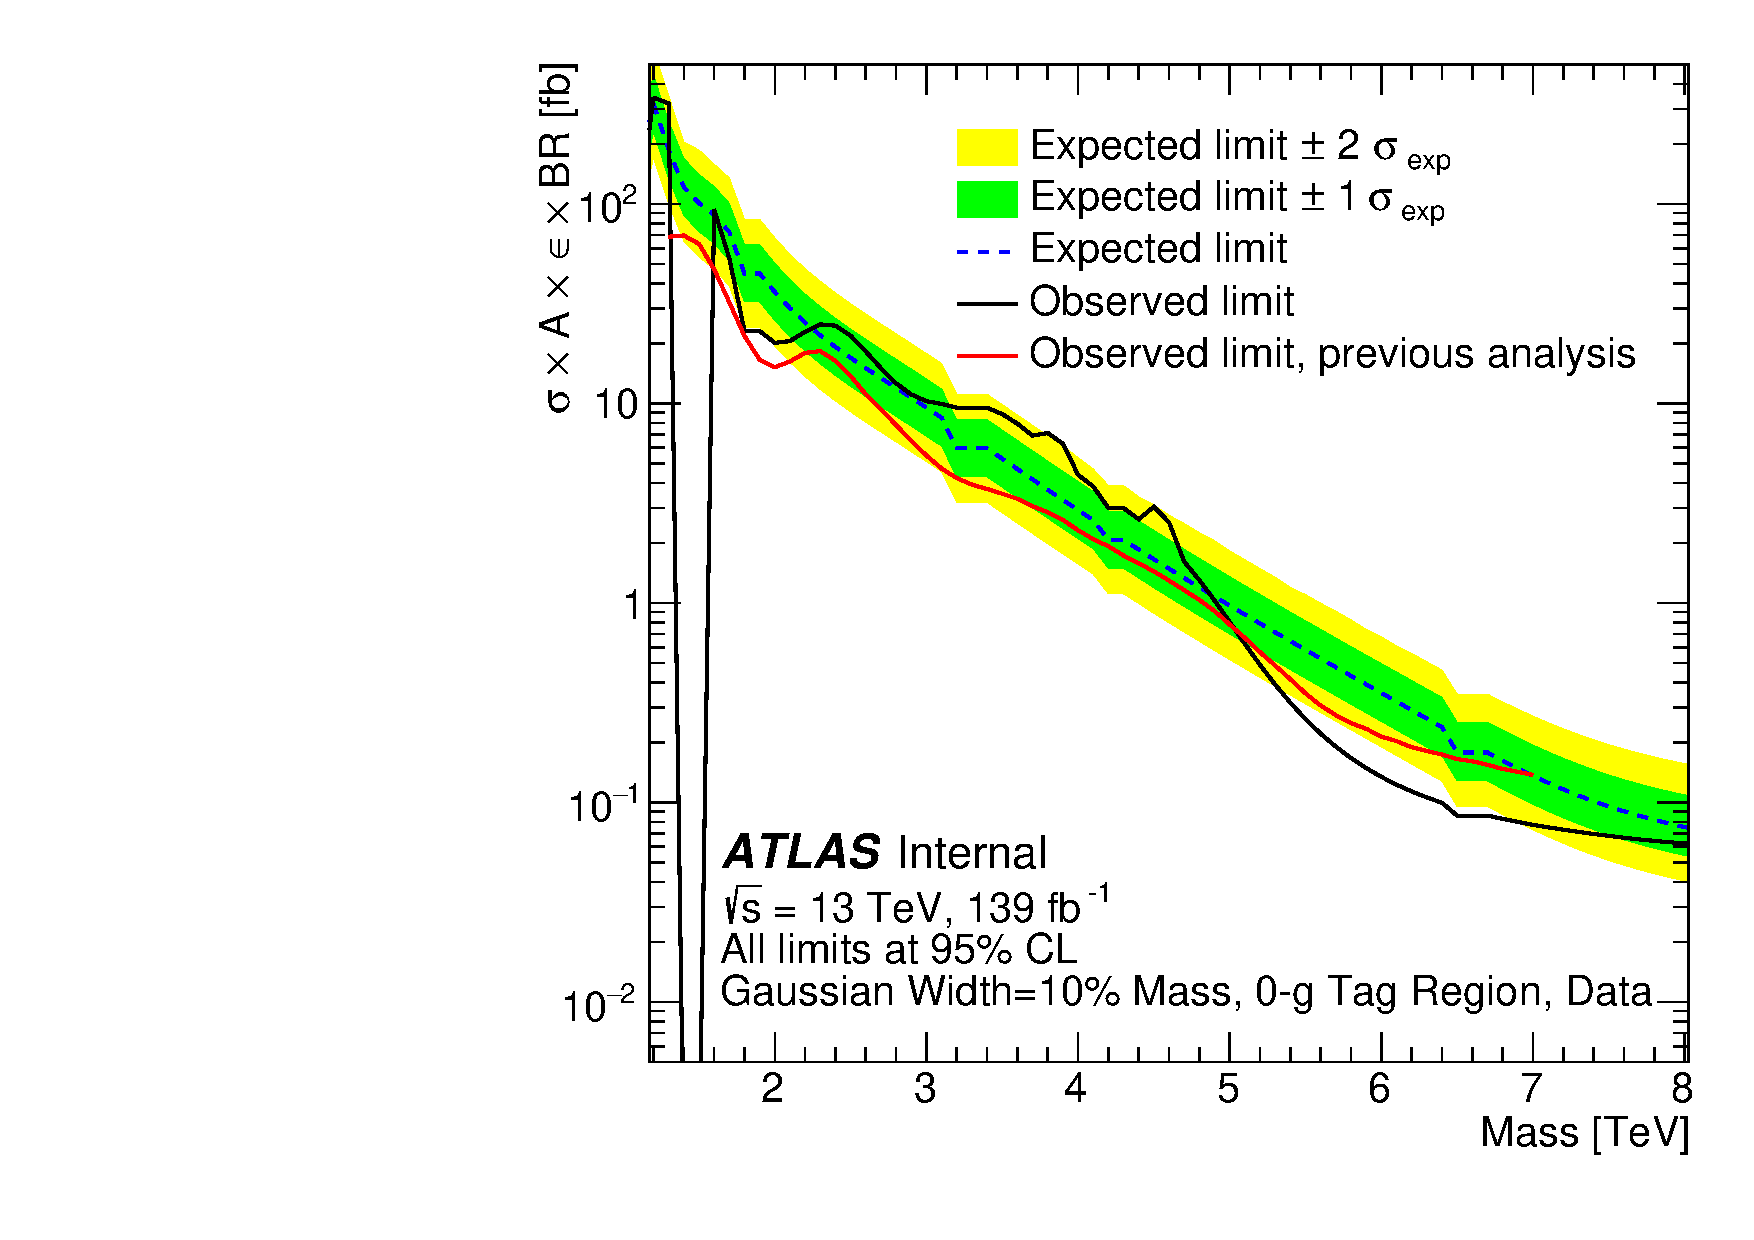
\includegraphics[width=0.3\textwidth]{figures/app-SignalIndependentLimits/Gauss_Limits_yStar0p8_Tag0_WidthPercent10_1200to8000_sigma.pdf}
            }
            \subfigure[15\% Width Gaussian Limits]{ 
%                \label{fig:SignalIndependentGaussianLimits_SubWidth15} % uncomment if label used. 
                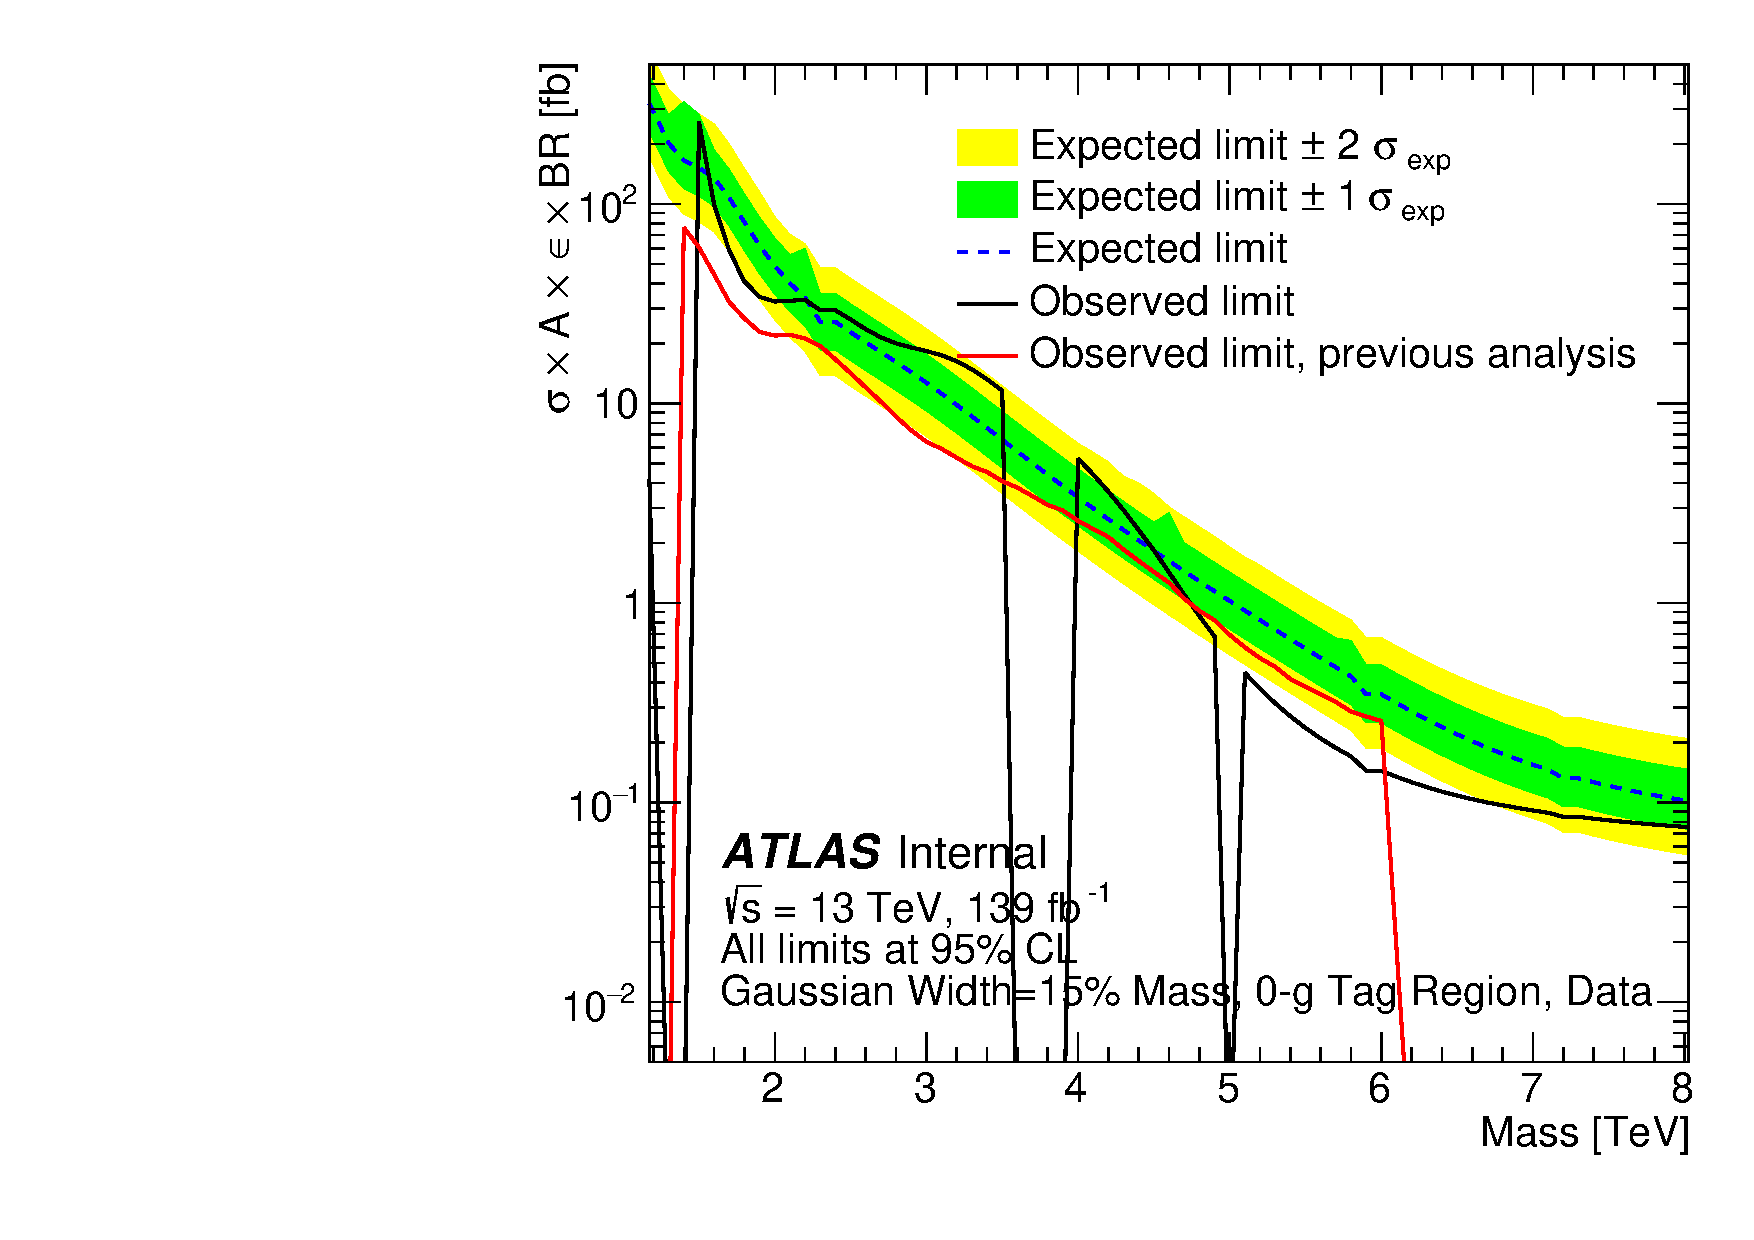
\includegraphics[width=0.3\textwidth]{figures/app-SignalIndependentLimits/Gauss_Limits_yStar0p8_Tag0_WidthPercent15_1200to8000_sigma.pdf}
            }
            \caption{Model-independent limits set in the untagged $y^{*} < 0.8$ Signal Region using Gaussian resonances of varying widths from 0\% to 15\% of their peak position without systematics included using the full 139fb$^{-1}$ Run-2 dataset.}
            \label{fig:SignalIndependentGaussianLimits_UntaggedYStar0p8}
        \end{figure}


        \begin{figure}[!htb]
            \subfigure[0\% Width Gaussian Limits]{ 
%                \label{fig:SignalIndependentGaussianLimits_SubWidth0} % uncomment if label used. 
                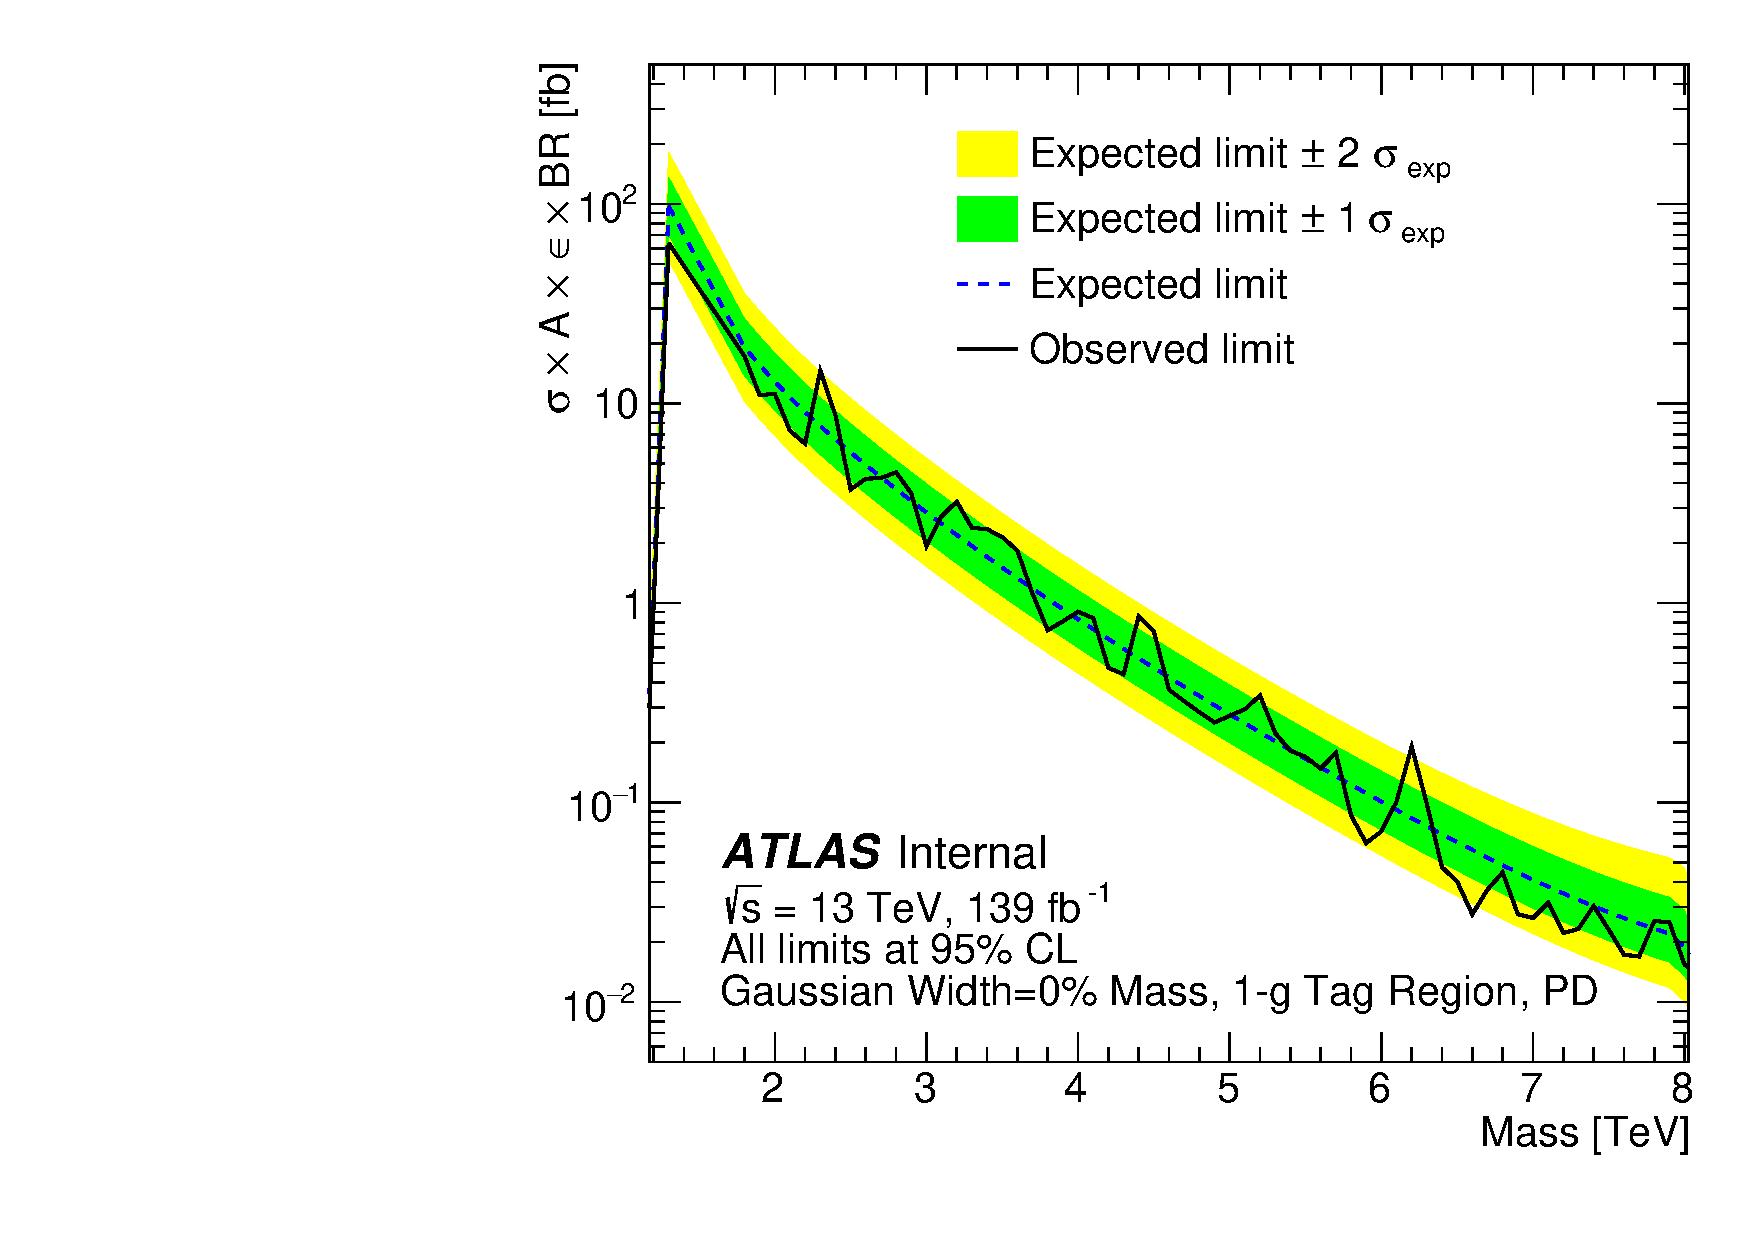
\includegraphics[width=0.3\textwidth]{figures/app-SignalIndependentLimits/Gauss_Limits_yStar0p6_Tag1_WidthPercent0_1200to8000_sigma.pdf}
            }
            \subfigure[3\% Width Gaussian Limits]{ 
%                \label{fig:SignalIndependentGaussianLimits_SubWidth3} % uncomment if label used. 
                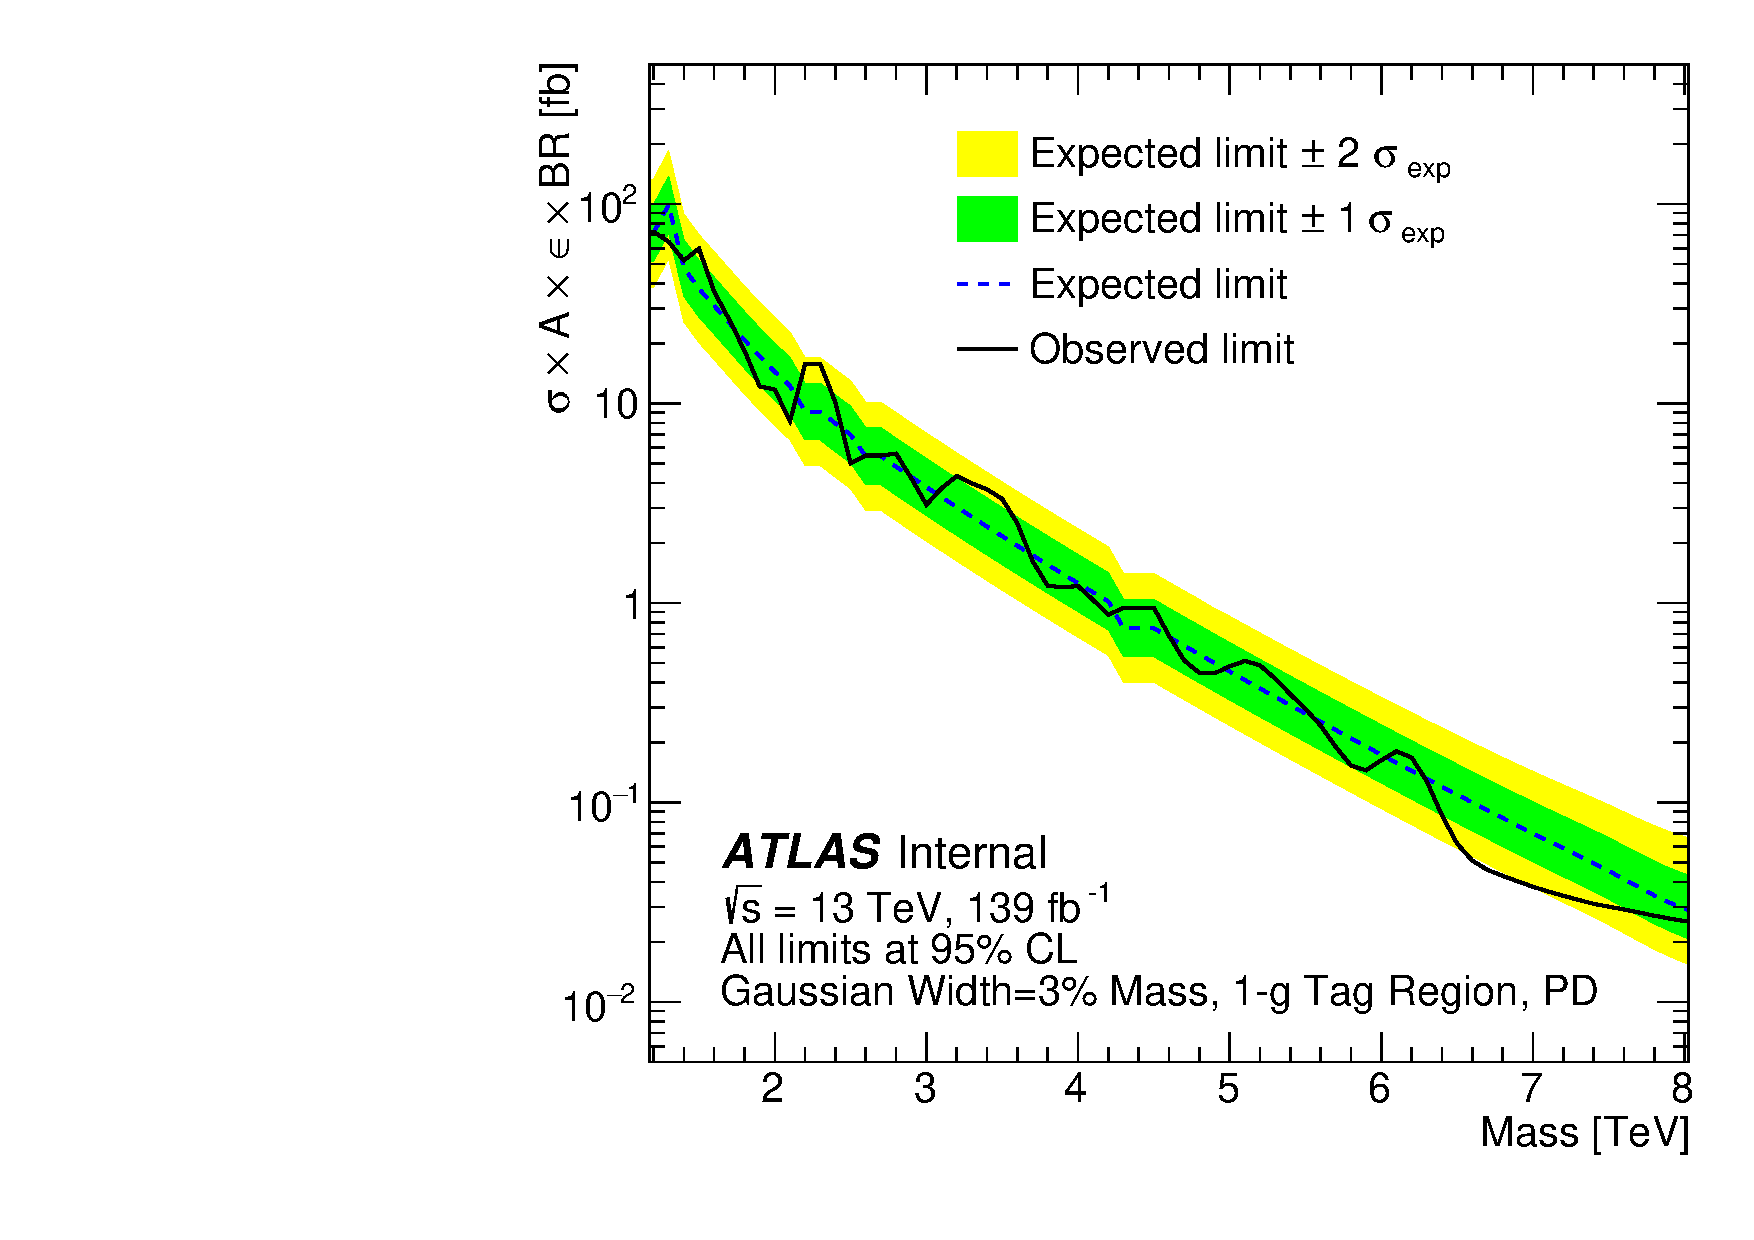
\includegraphics[width=0.3\textwidth]{figures/app-SignalIndependentLimits/Gauss_Limits_yStar0p6_Tag1_WidthPercent3_1200to8000_sigma.pdf}
            }
            \subfigure[5\% Width Gaussian Limits]{ 
%                \label{fig:SignalIndependentGaussianLimits_SubWidth5} % uncomment if label used. 
                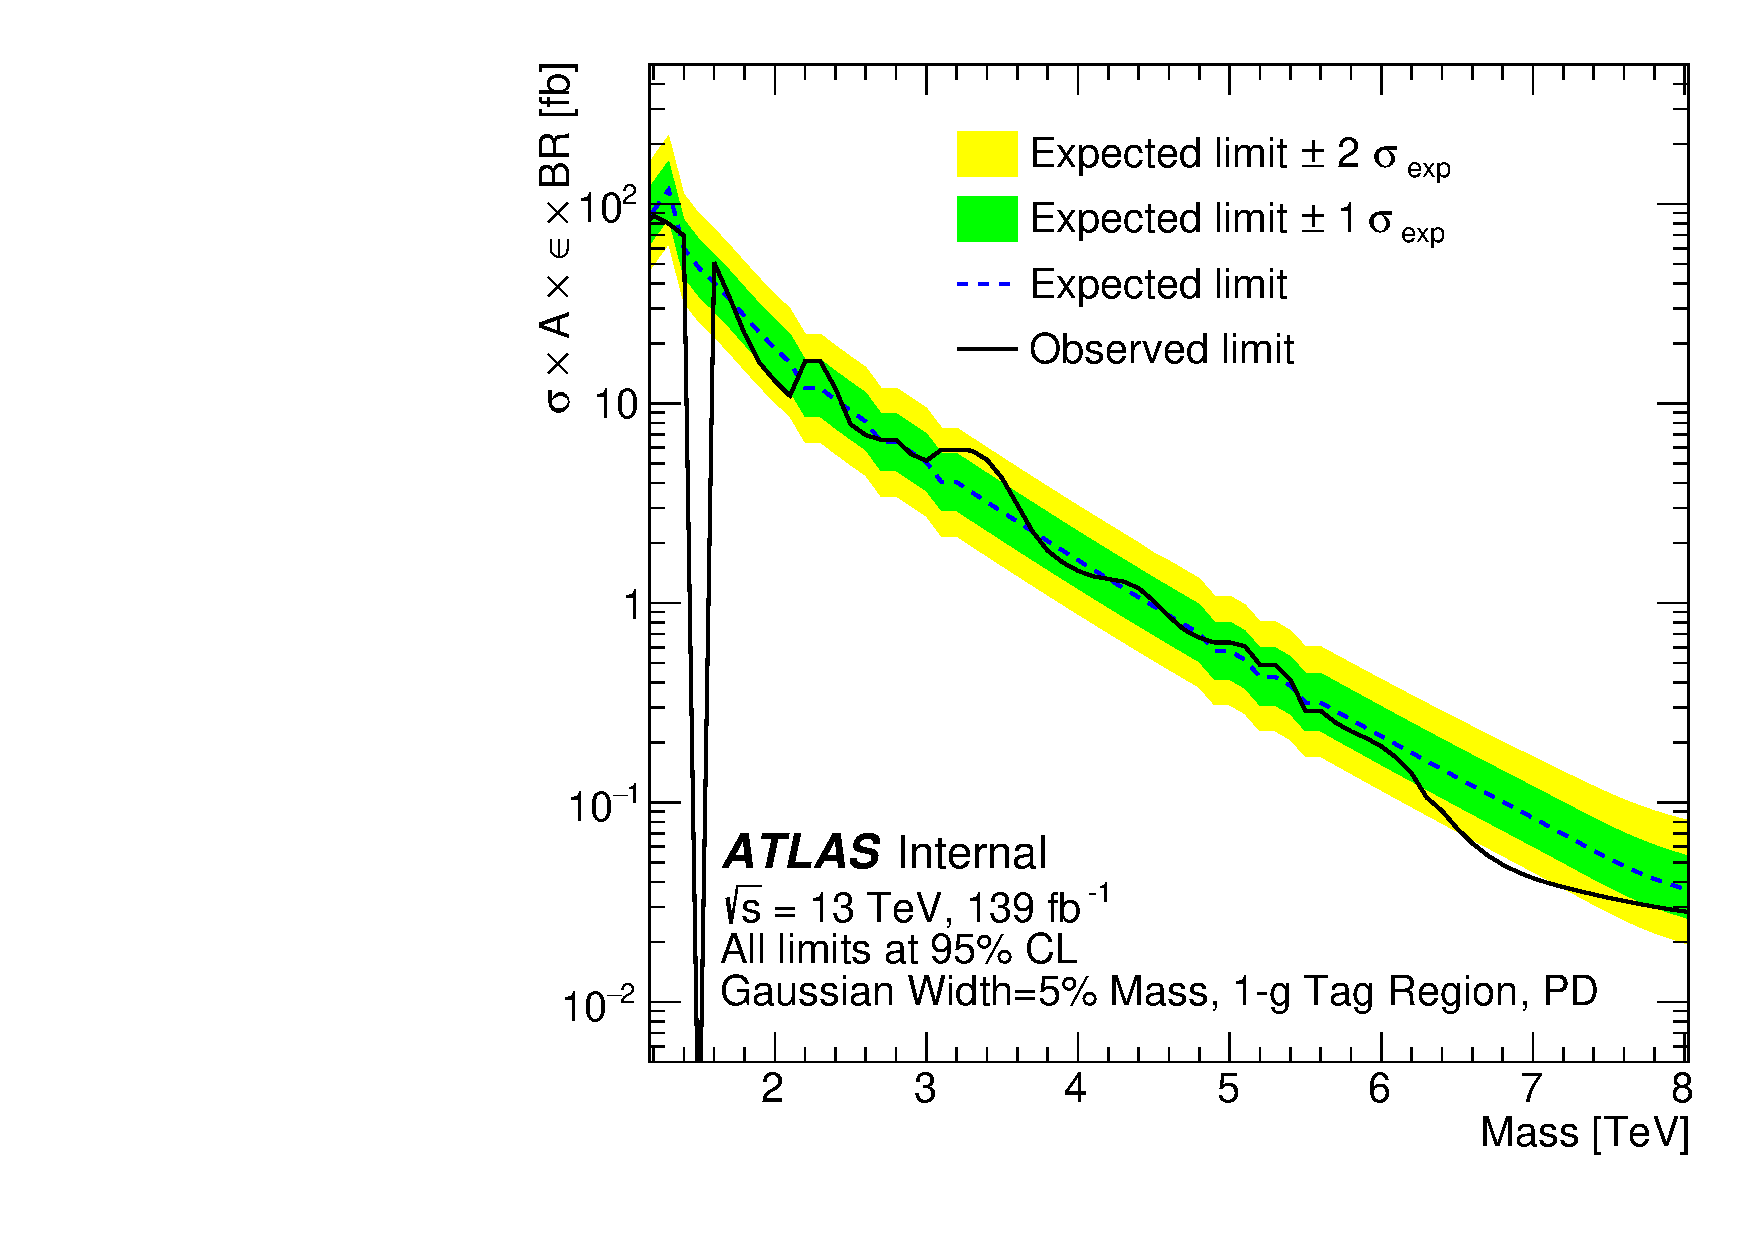
\includegraphics[width=0.3\textwidth]{figures/app-SignalIndependentLimits/Gauss_Limits_yStar0p6_Tag1_WidthPercent5_1200to8000_sigma.pdf}
            }
            \subfigure[7\% Width Gaussian Limits]{ 
%                \label{fig:SignalIndependentGaussianLimits_SubWidth7} % uncomment if label used. 
                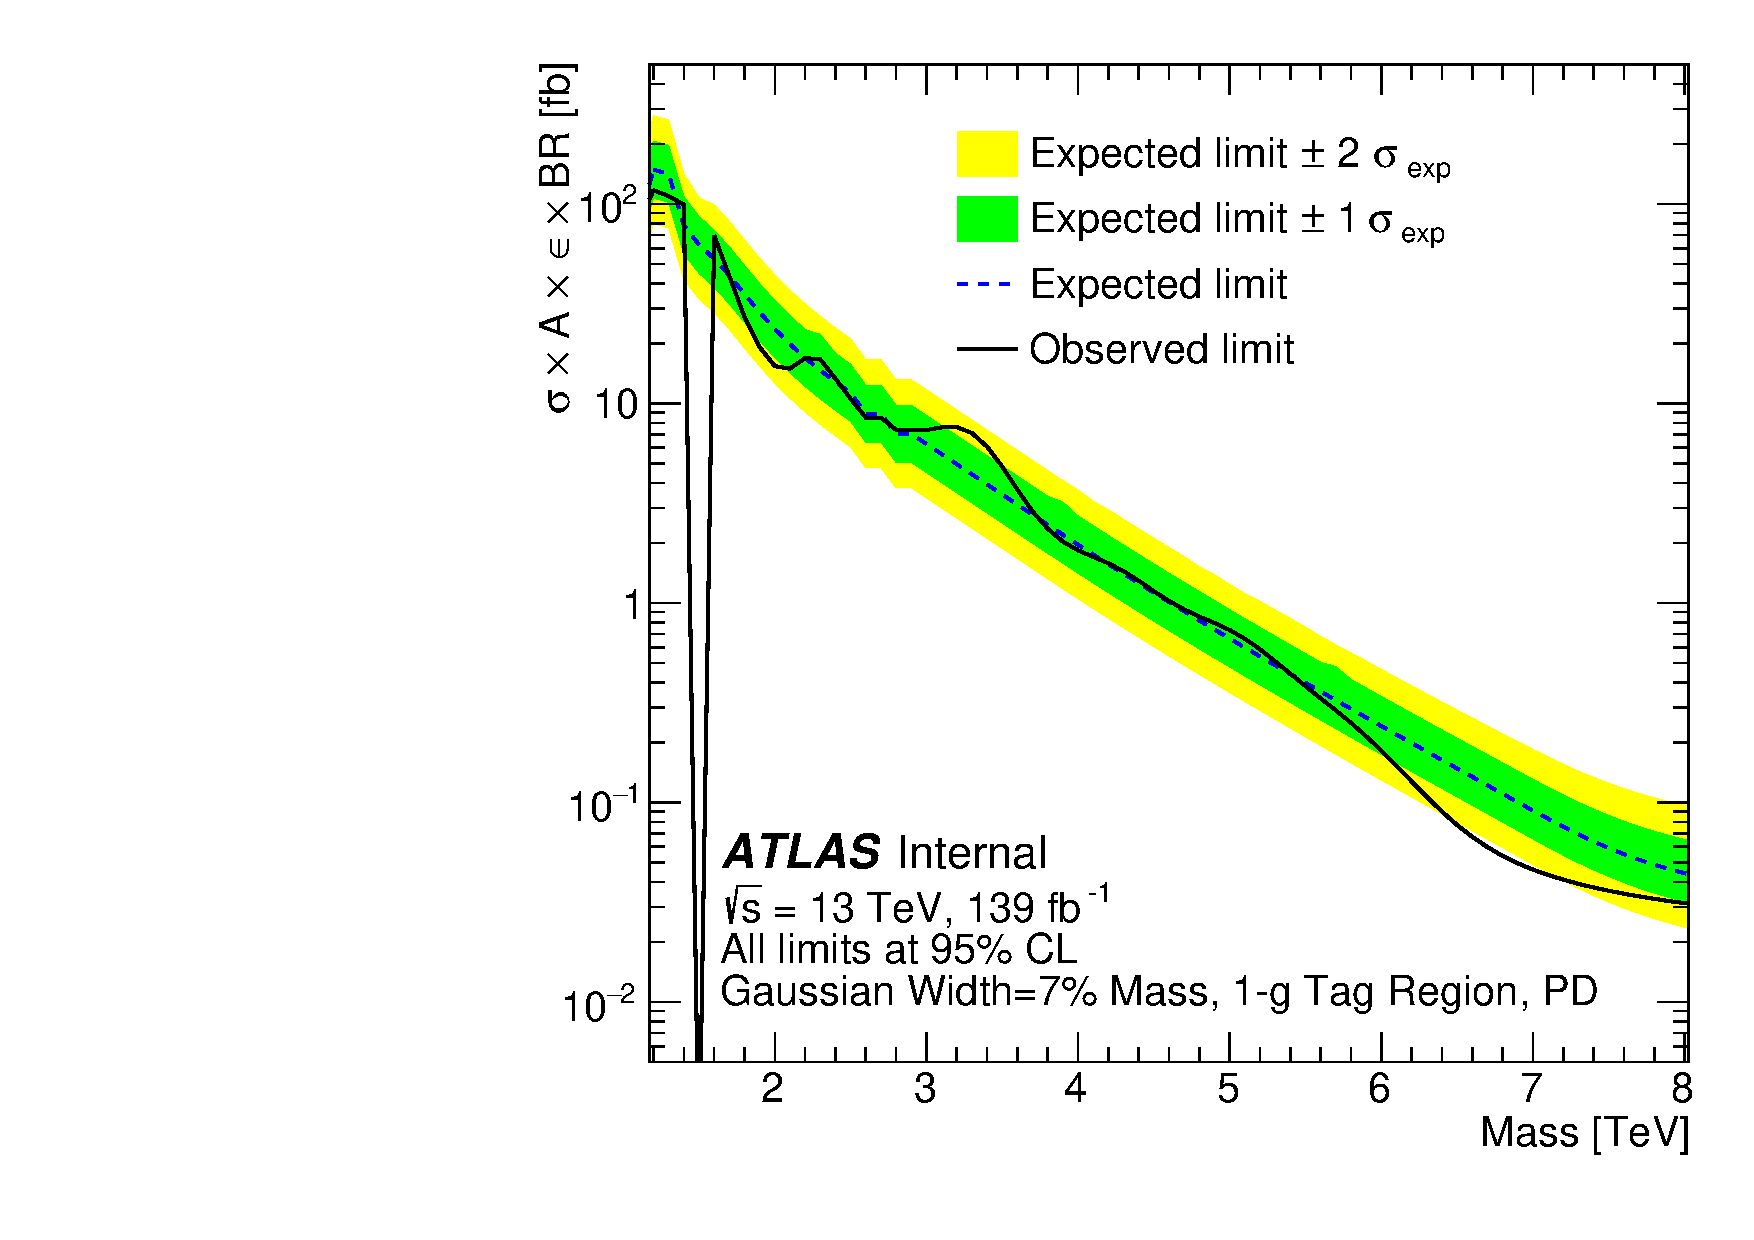
\includegraphics[width=0.3\textwidth]{figures/app-SignalIndependentLimits/Gauss_Limits_yStar0p6_Tag1_WidthPercent7_1200to8000_sigma.pdf}
            }
            \subfigure[10\% Width Gaussian Limits]{ 
%                \label{fig:SignalIndependentGaussianLimits_SubWidth10} % uncomment if label used. 
                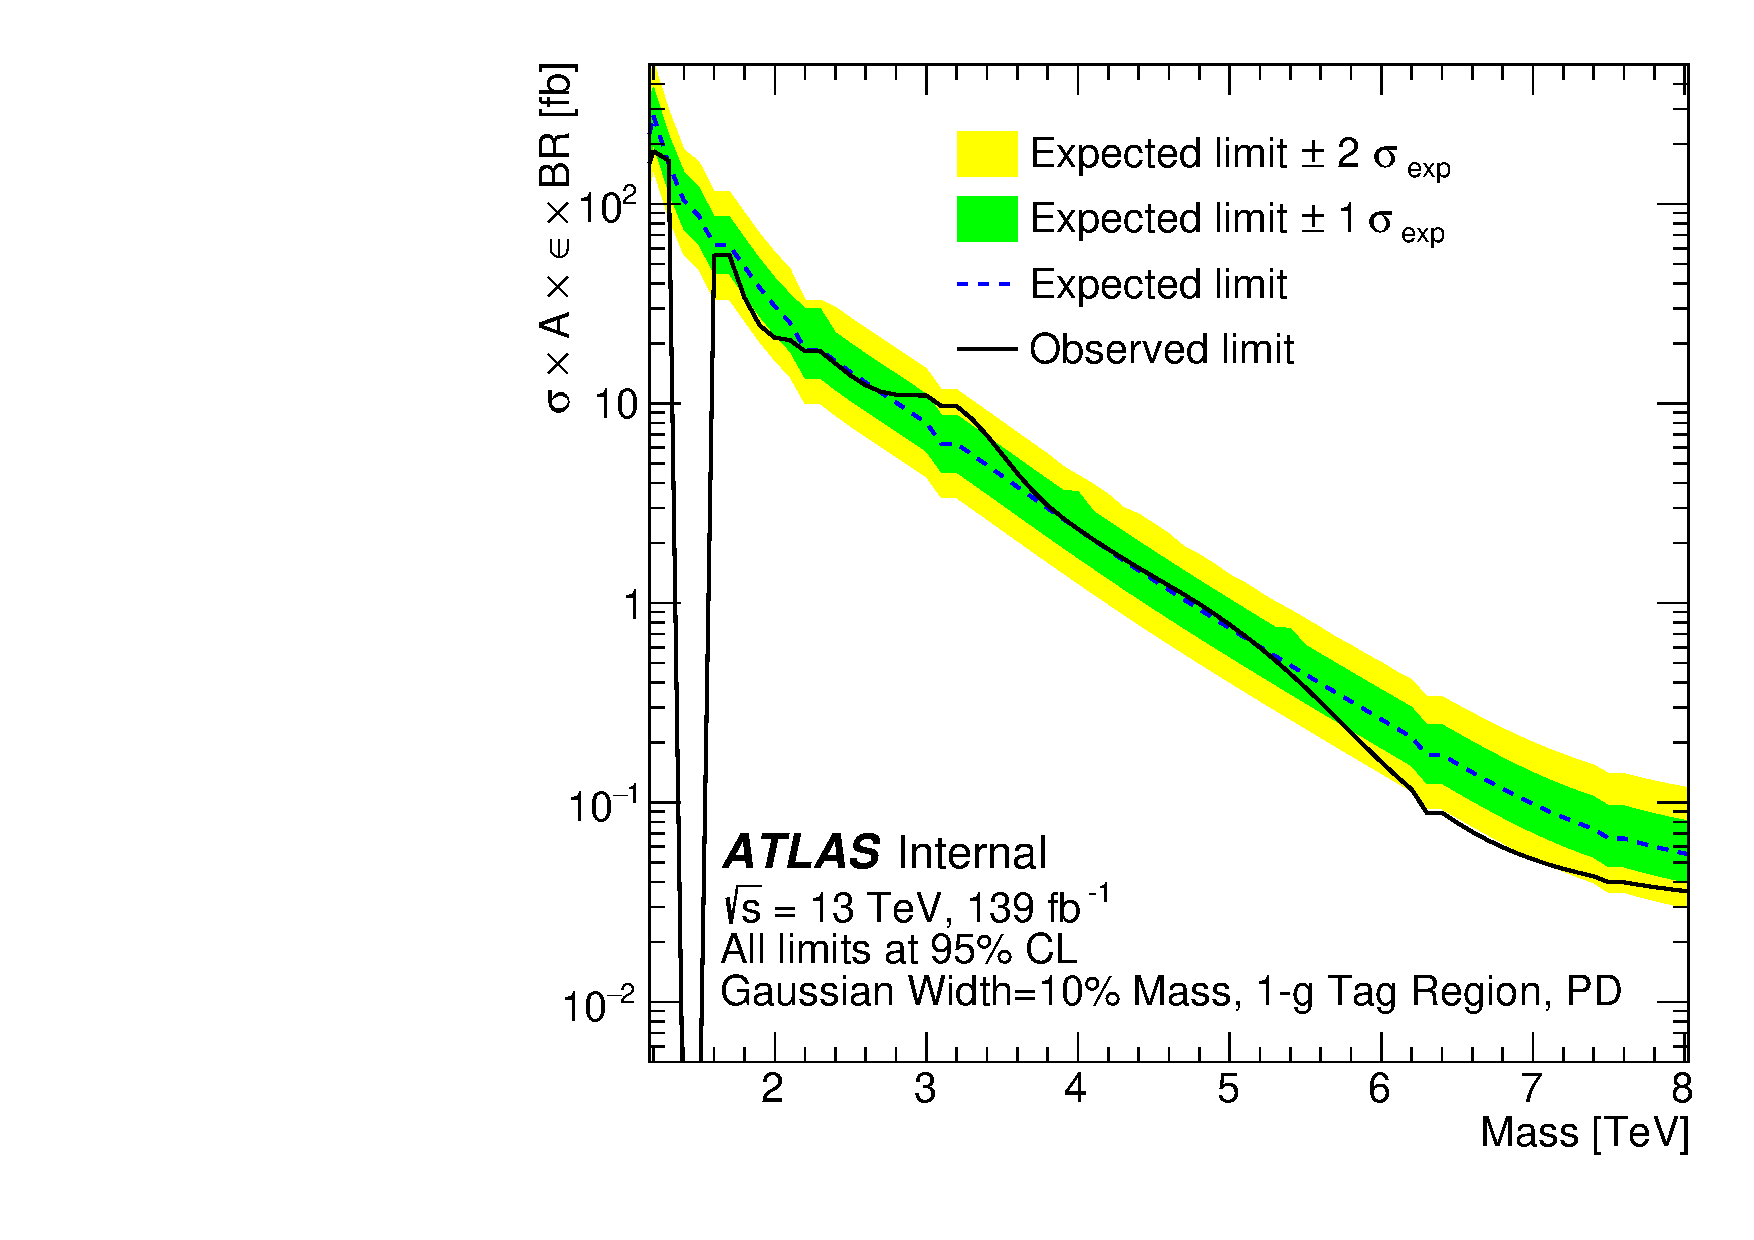
\includegraphics[width=0.3\textwidth]{figures/app-SignalIndependentLimits/Gauss_Limits_yStar0p6_Tag1_WidthPercent10_1200to8000_sigma.pdf}
            }
            \subfigure[15\% Width Gaussian Limits]{ 
%                \label{fig:SignalIndependentGaussianLimits_SubWidth15} % uncomment if label used. 
                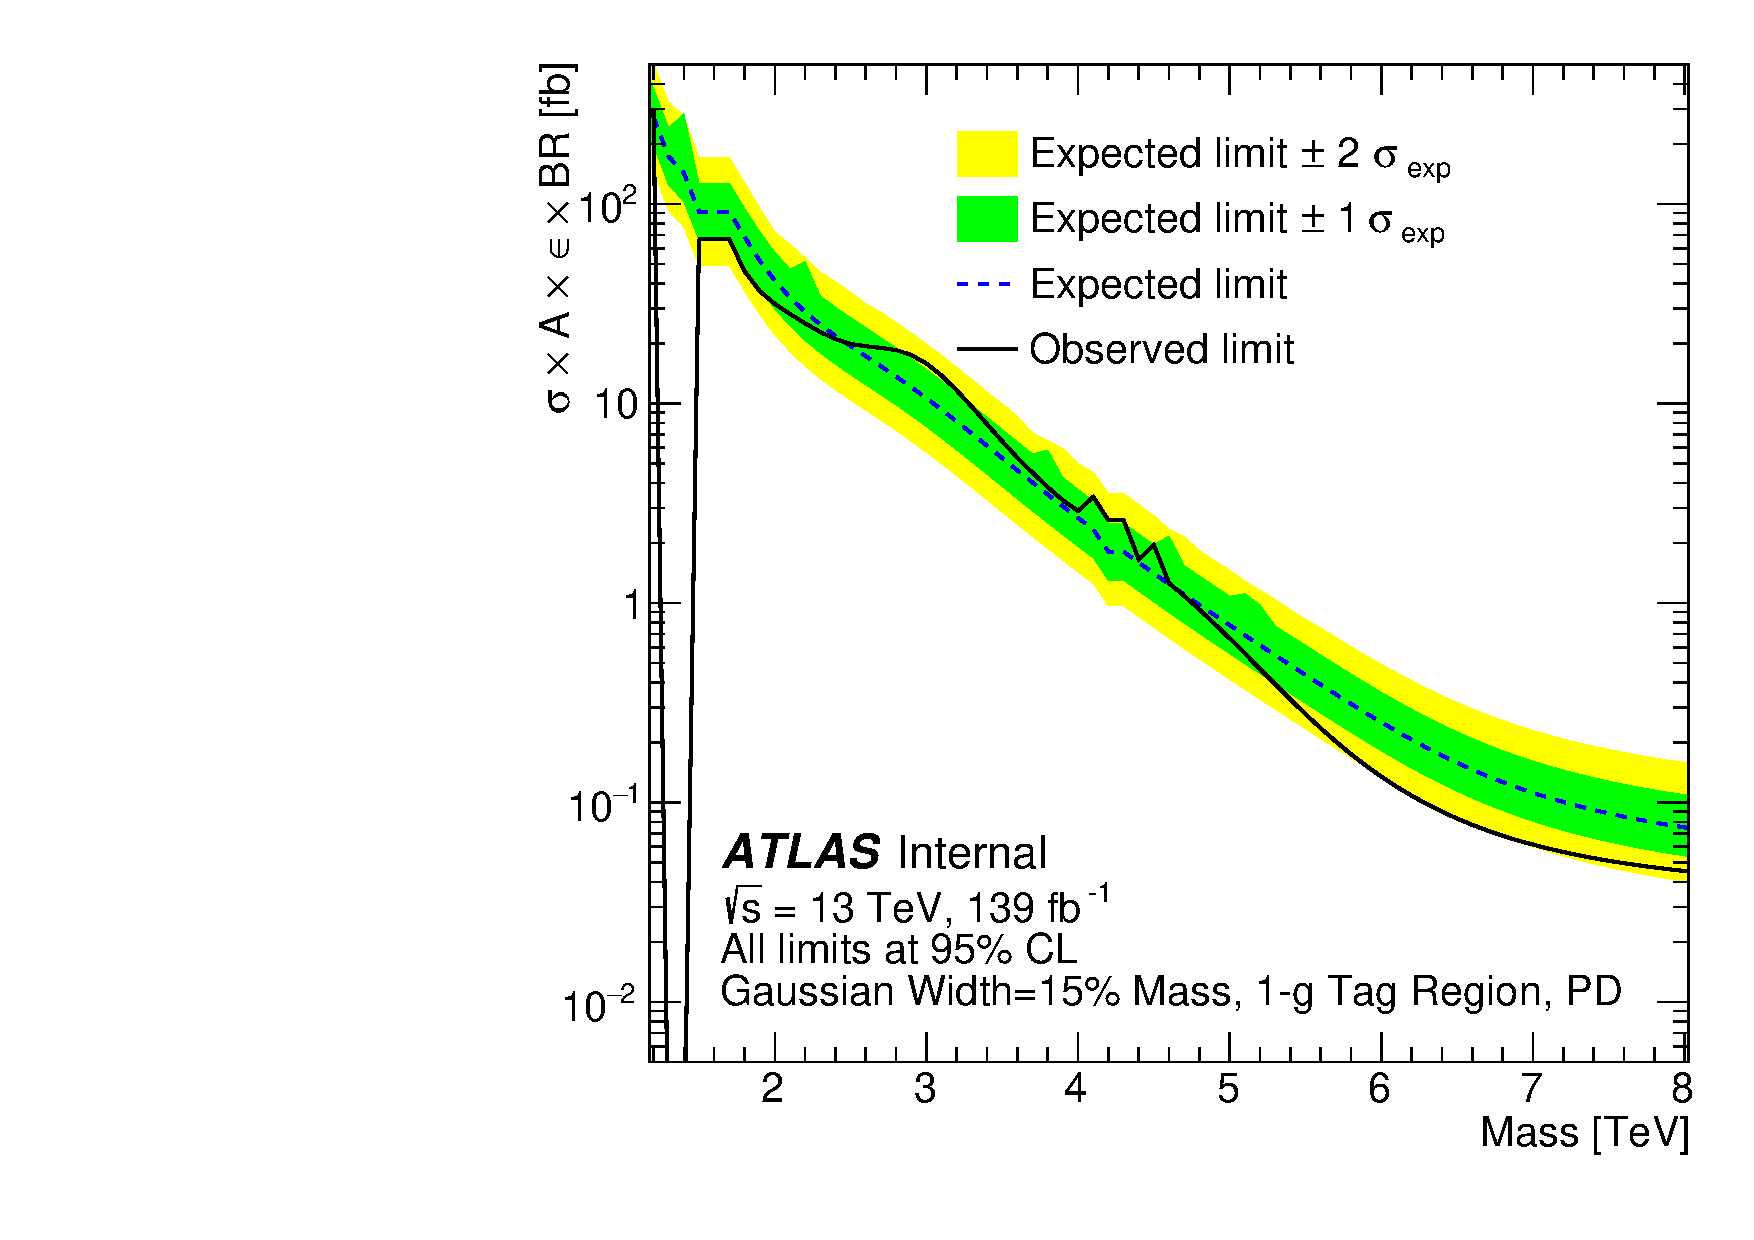
\includegraphics[width=0.3\textwidth]{figures/app-SignalIndependentLimits/Gauss_Limits_yStar0p6_Tag1_WidthPercent15_1200to8000_sigma.pdf}
            }
            \caption{Model-independent limits set in the 1-$g$ tagged $y^{*} < 0.6$ Signal Region using Gaussian resonances of varying widths from 0\% to 15\% of their peak position without systematics included using the full 139fb$^{-1}$ Run-2 dataset.}
            \label{fig:SignalIndependentGaussianLimits_1gYStar0p6}
        \end{figure}

        \begin{figure}[!htb]
            \subfigure[0\% Width Gaussian Limits]{ 
%                \label{fig:SignalIndependentGaussianLimits_SubWidth0} % uncomment if label used. 
                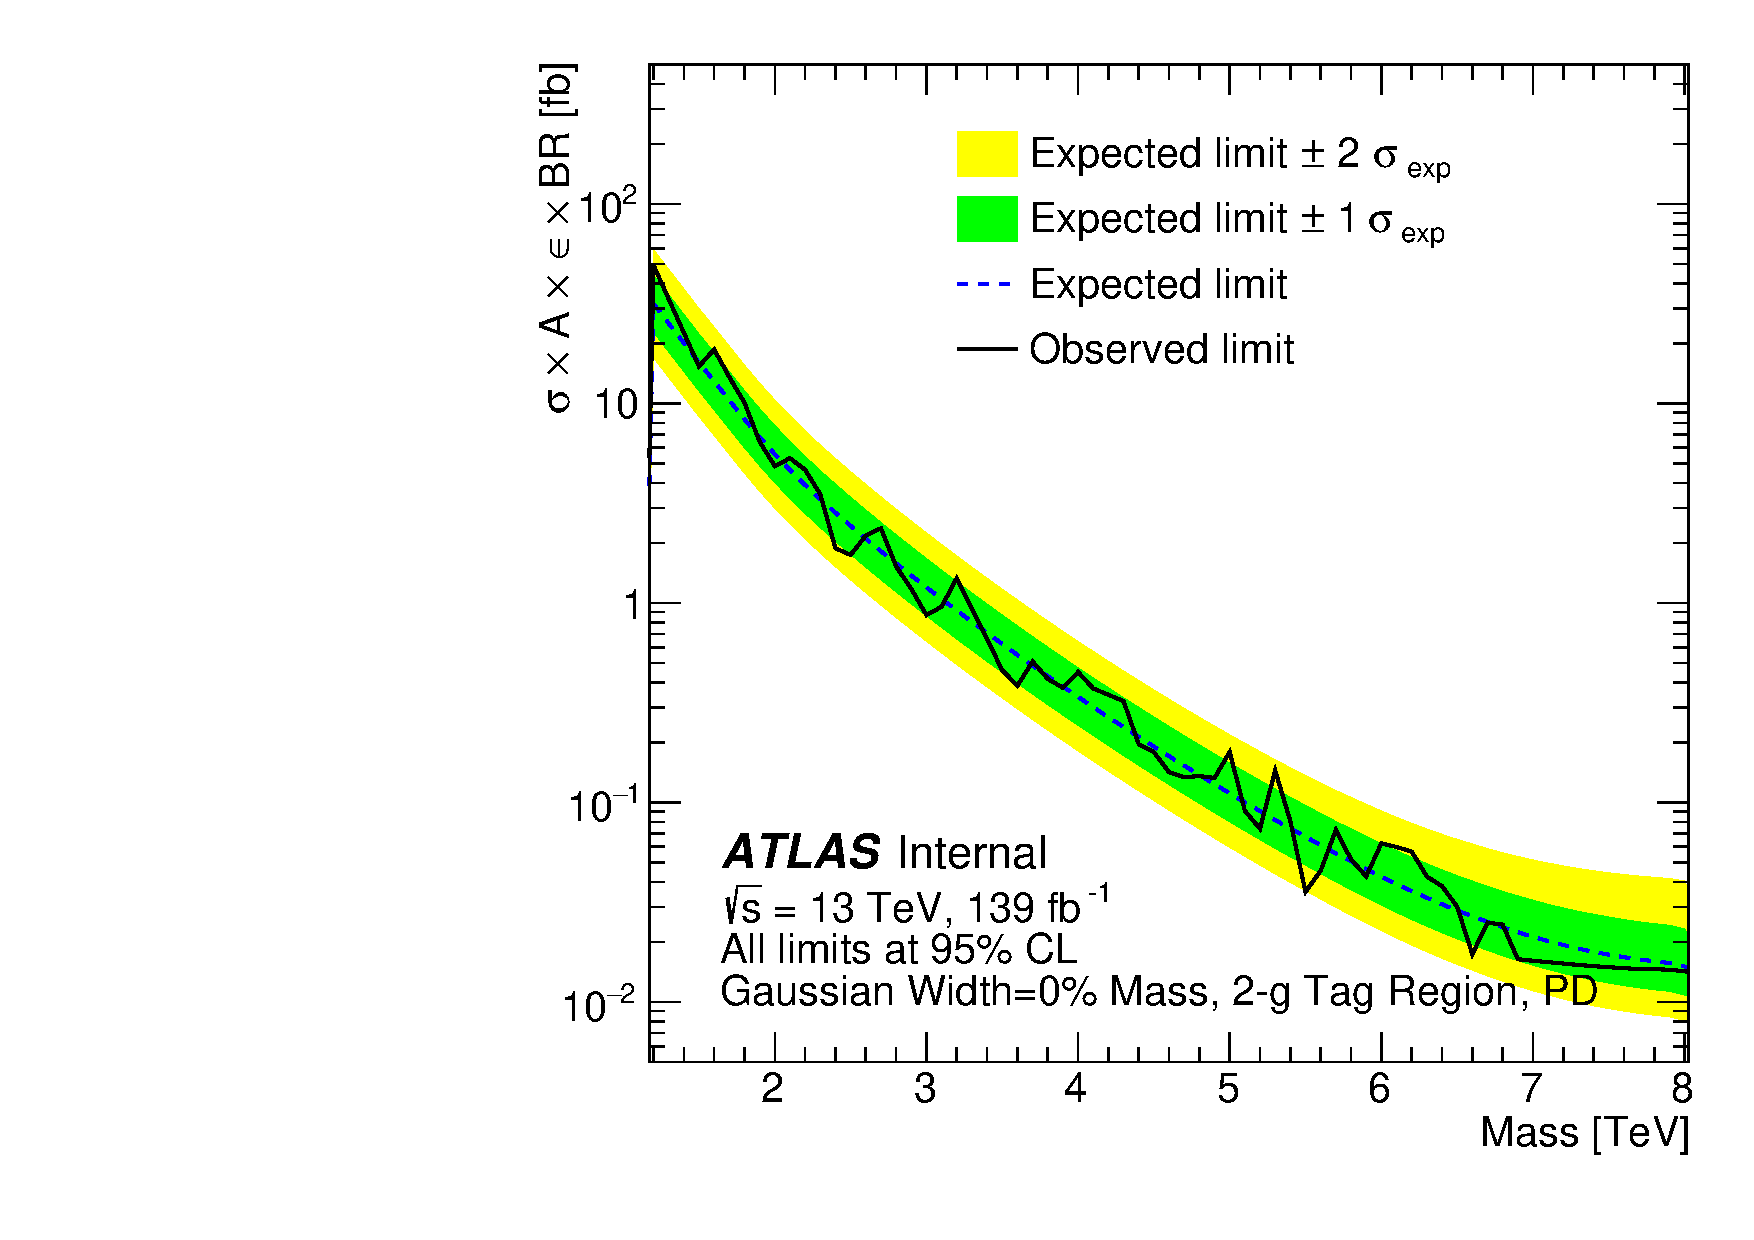
\includegraphics[width=0.3\textwidth]{figures/app-SignalIndependentLimits/Gauss_Limits_yStar0p8_Tag2_WidthPercent0_1200to8000_sigma.pdf}
            }
            \subfigure[3\% Width Gaussian Limits]{ 
%                \label{fig:SignalIndependentGaussianLimits_SubWidth3} % uncomment if label used. 
                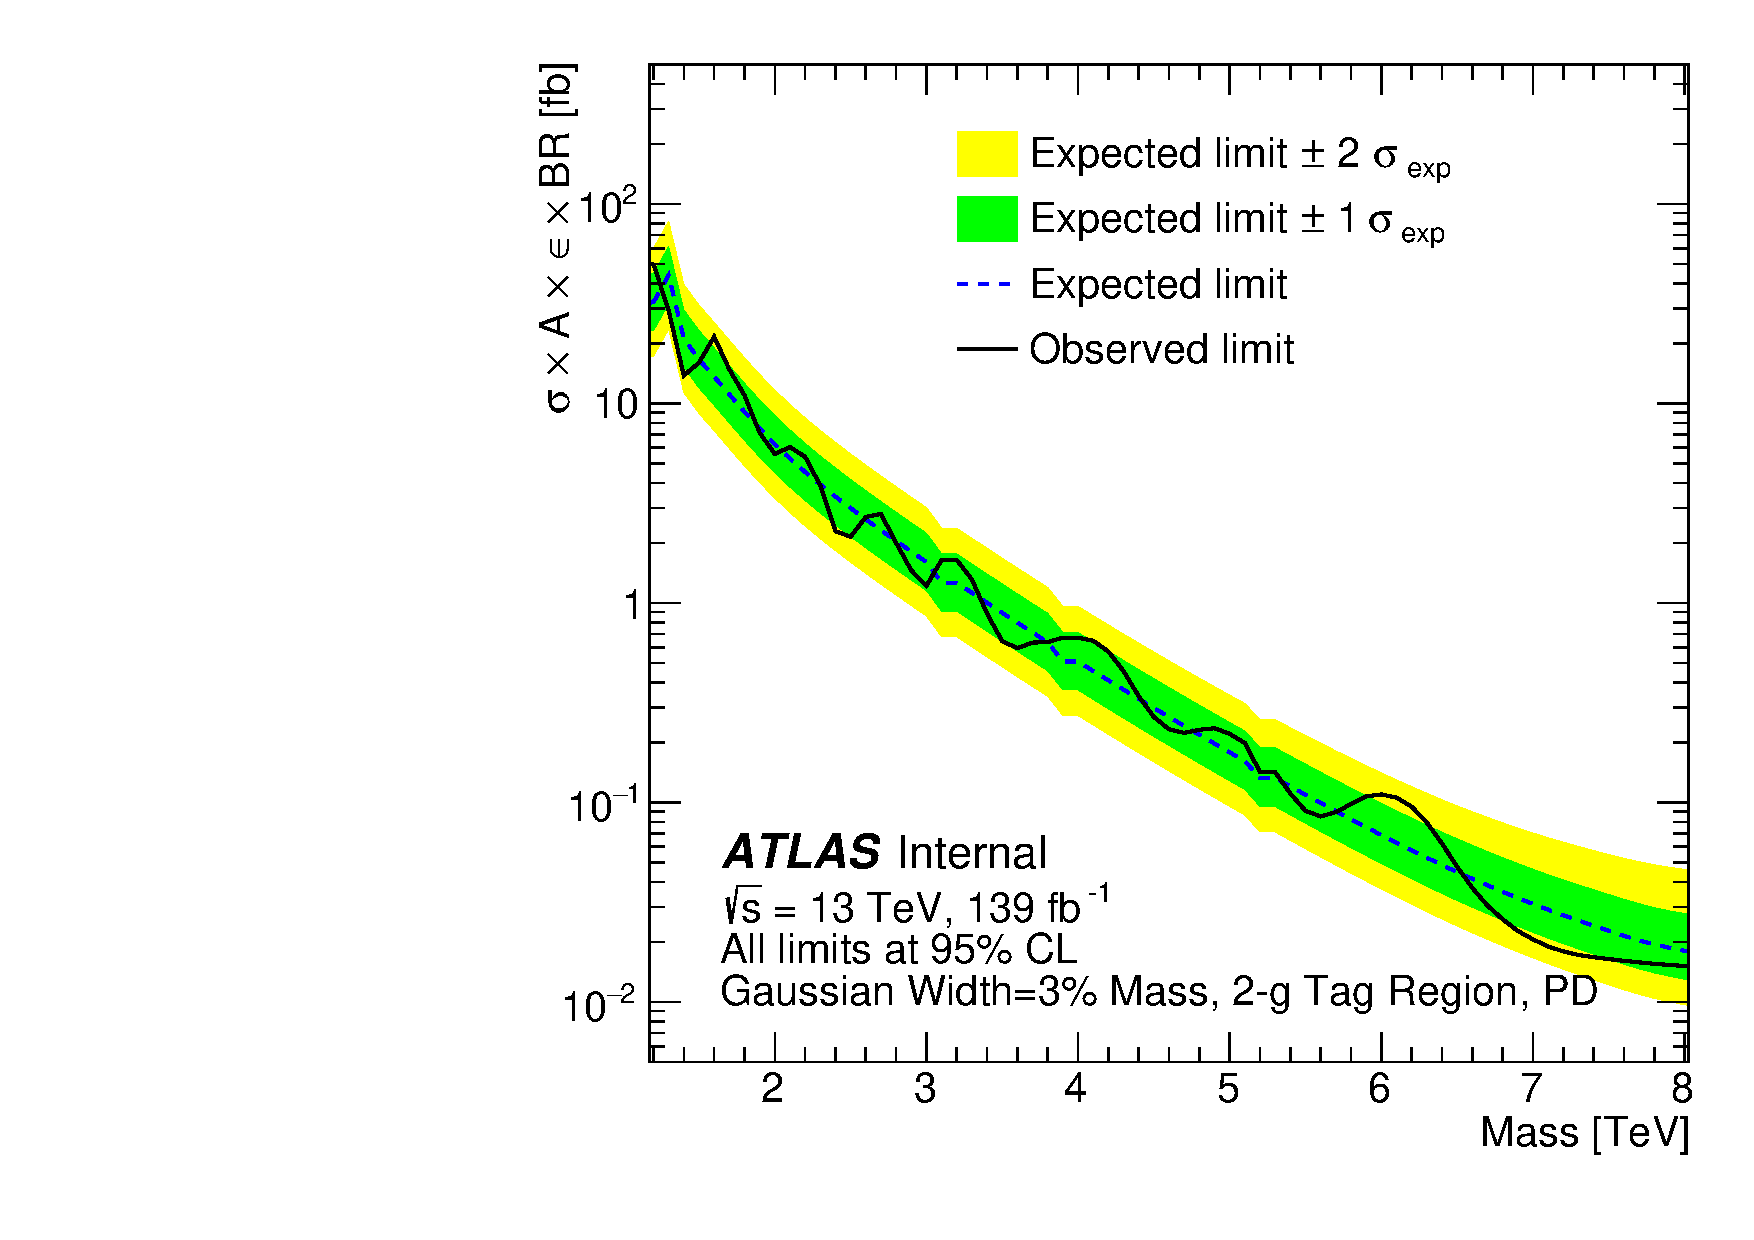
\includegraphics[width=0.3\textwidth]{figures/app-SignalIndependentLimits/Gauss_Limits_yStar0p8_Tag2_WidthPercent3_1200to8000_sigma.pdf}
            }
            \subfigure[5\% Width Gaussian Limits]{ 
%                \label{fig:SignalIndependentGaussianLimits_SubWidth5} % uncomment if label used. 
                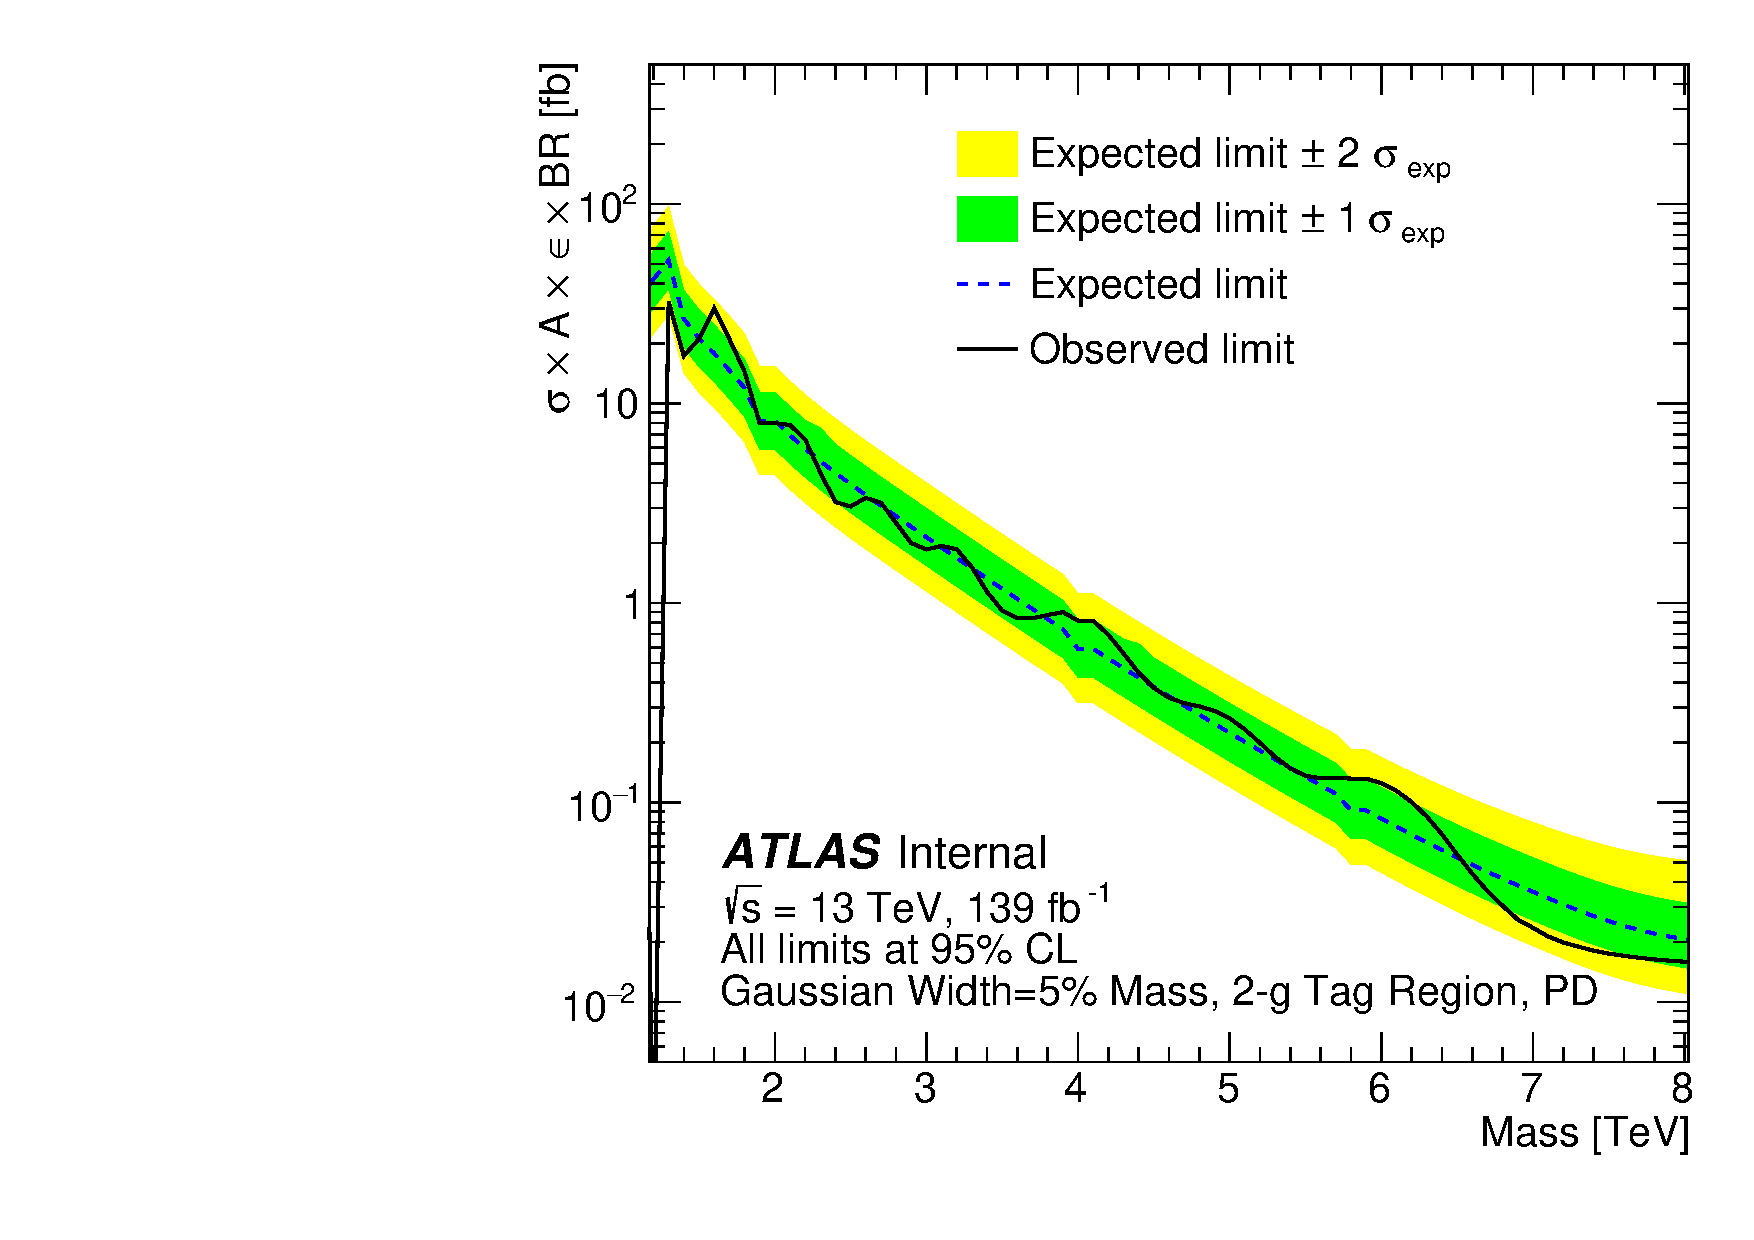
\includegraphics[width=0.3\textwidth]{figures/app-SignalIndependentLimits/Gauss_Limits_yStar0p8_Tag2_WidthPercent5_1200to8000_sigma.pdf}
            }
            \subfigure[7\% Width Gaussian Limits]{ 
%                \label{fig:SignalIndependentGaussianLimits_SubWidth7} % uncomment if label used. 
                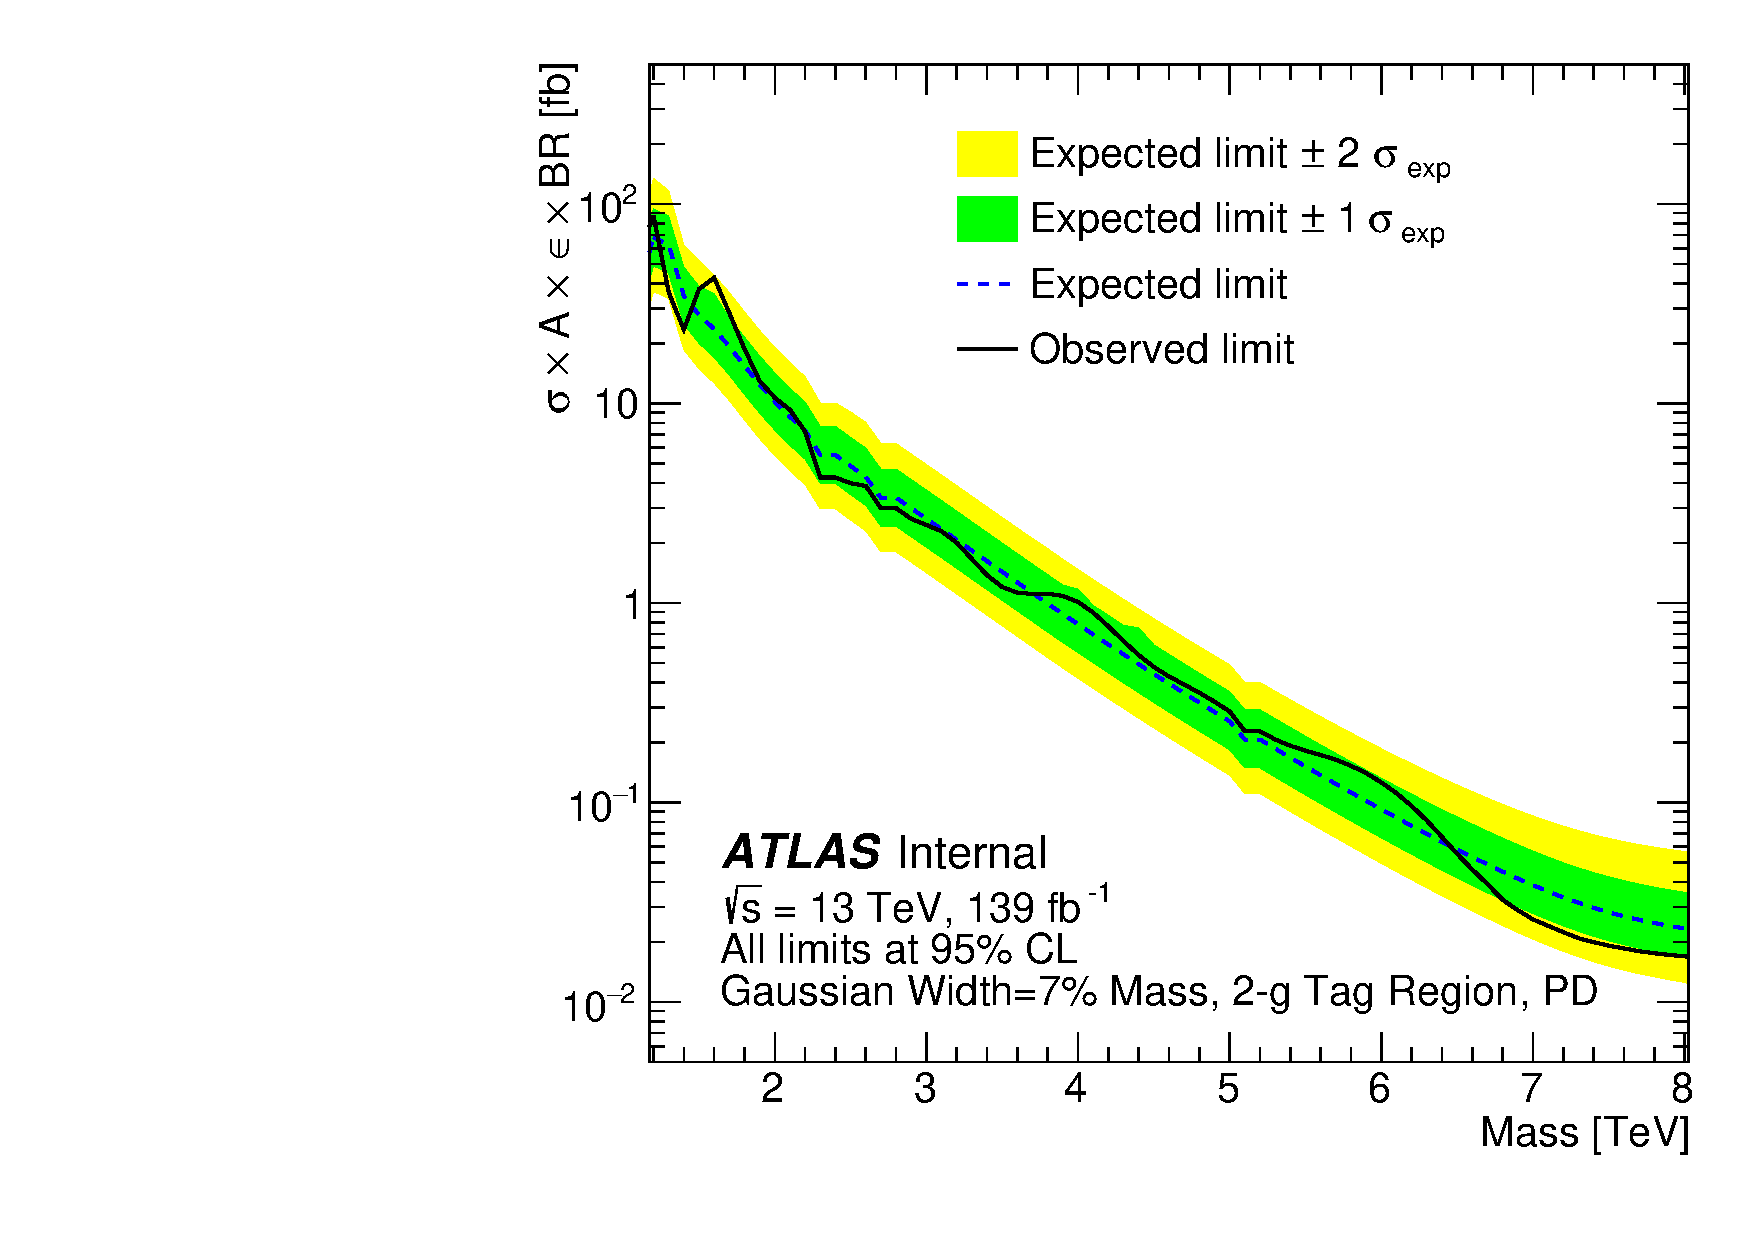
\includegraphics[width=0.3\textwidth]{figures/app-SignalIndependentLimits/Gauss_Limits_yStar0p8_Tag2_WidthPercent7_1200to8000_sigma.pdf}
            }
            \subfigure[10\% Width Gaussian Limits]{ 
%                \label{fig:SignalIndependentGaussianLimits_SubWidth10} % uncomment if label used. 
                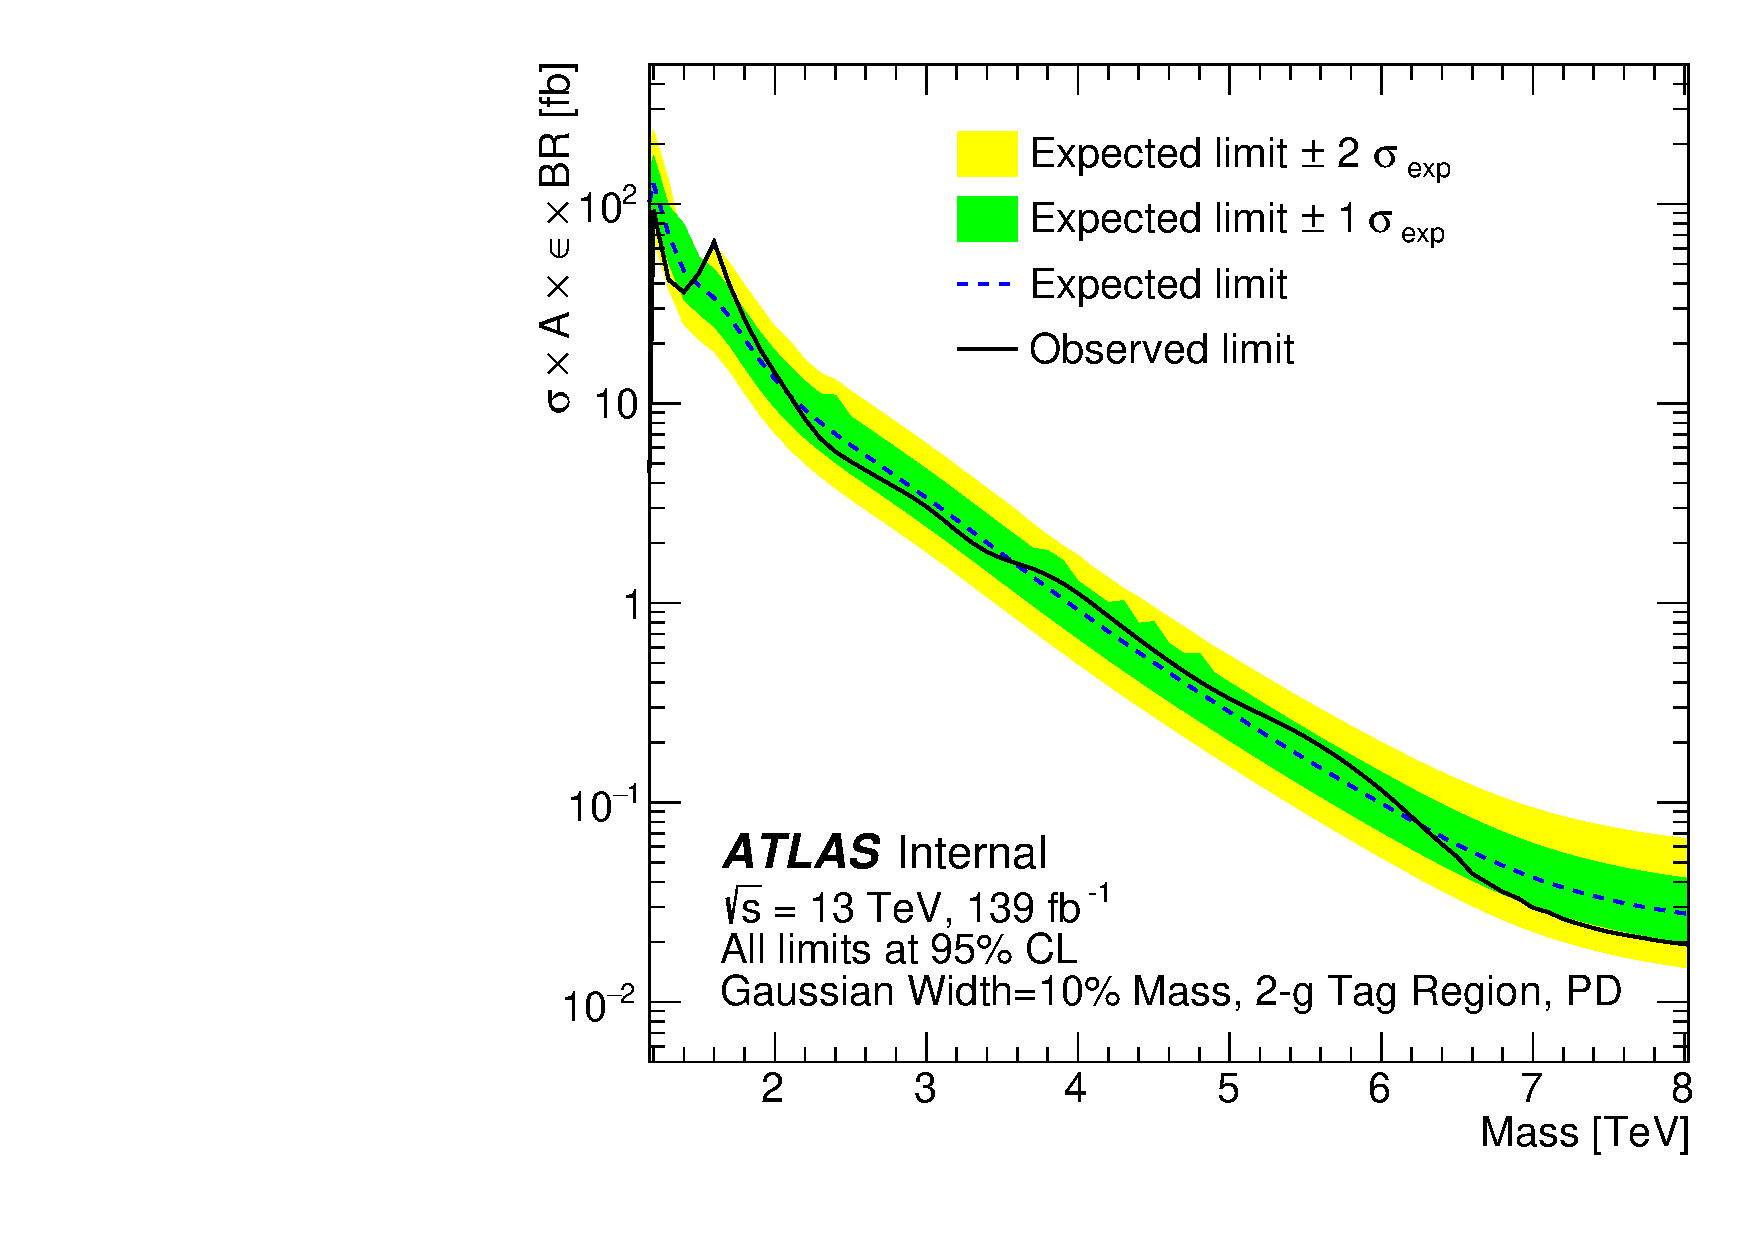
\includegraphics[width=0.3\textwidth]{figures/app-SignalIndependentLimits/Gauss_Limits_yStar0p8_Tag2_WidthPercent10_1200to8000_sigma.pdf}
            }
            \subfigure[15\% Width Gaussian Limits]{ 
%                \label{fig:SignalIndependentGaussianLimits_SubWidth15} % uncomment if label used. 
                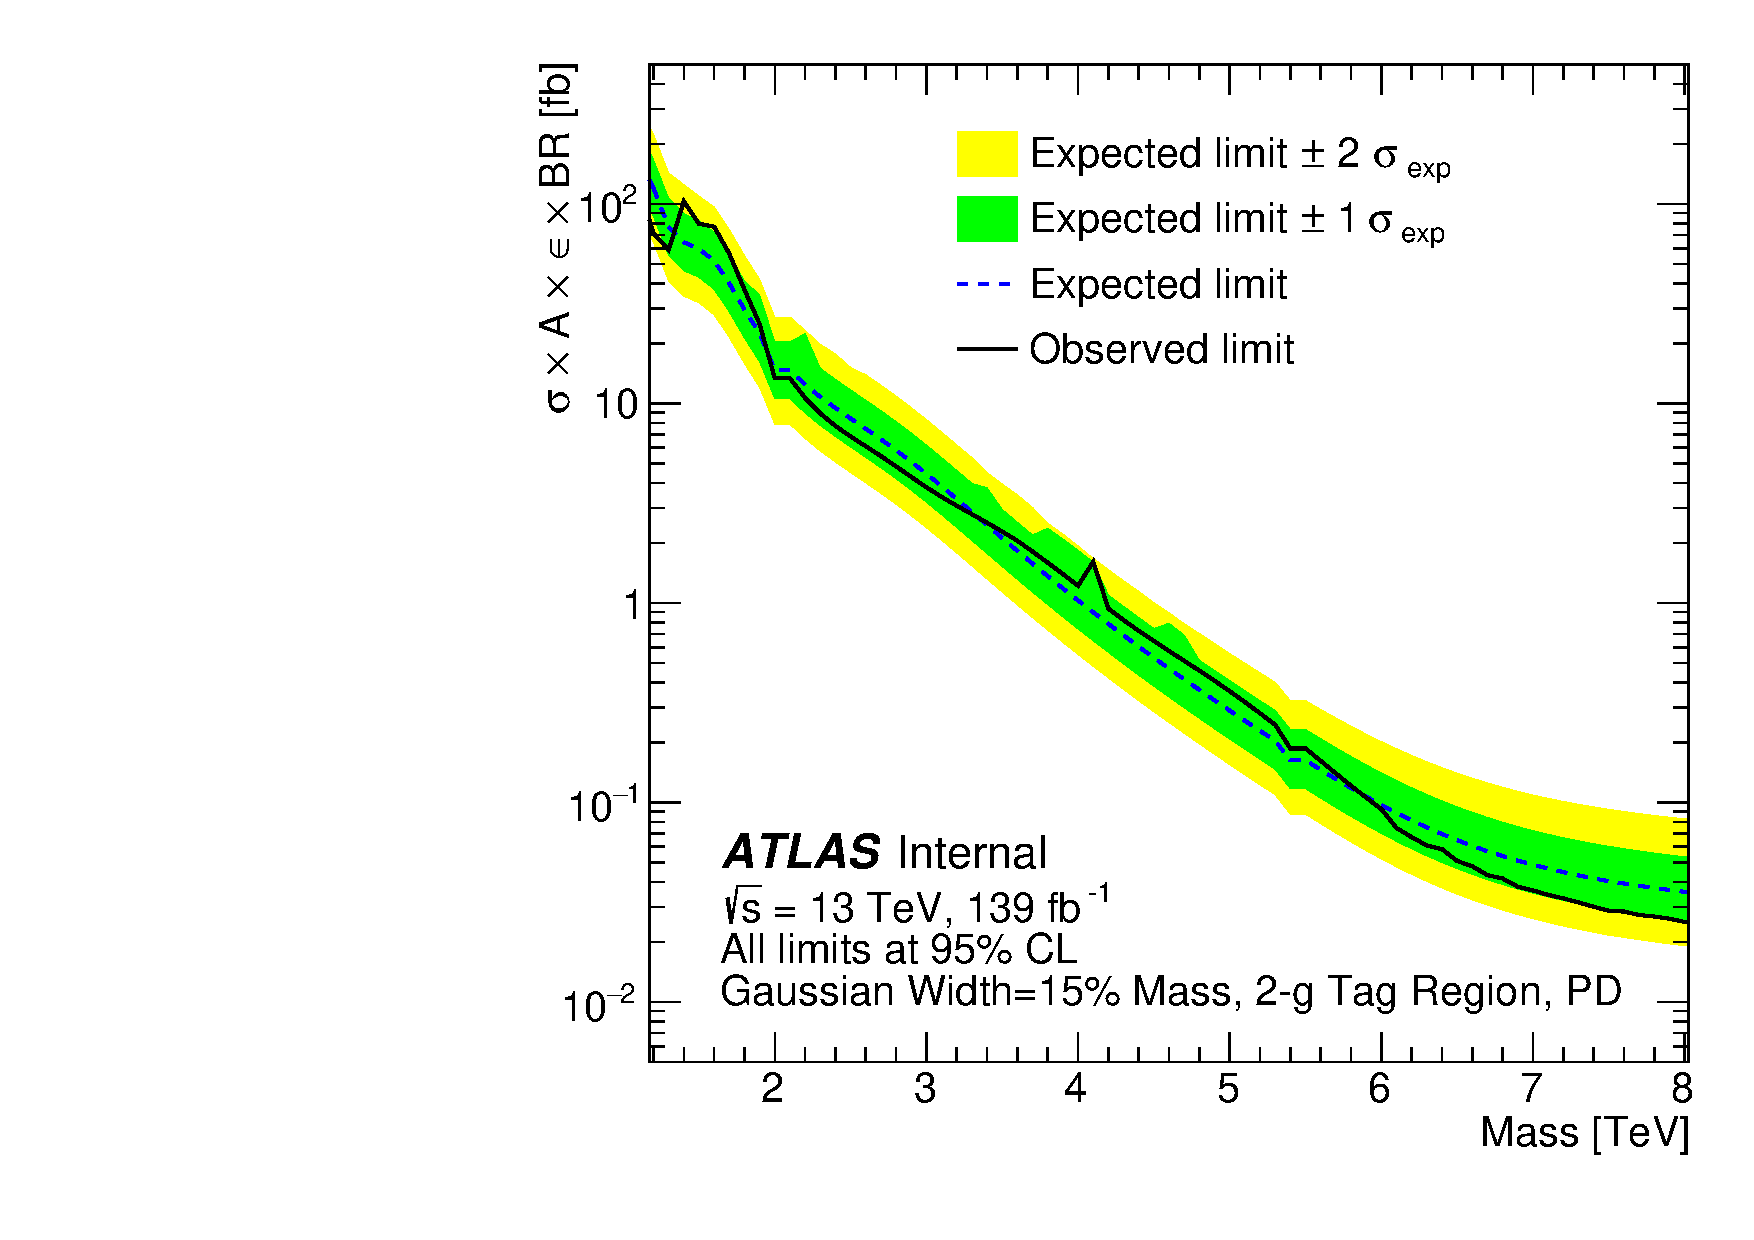
\includegraphics[width=0.3\textwidth]{figures/app-SignalIndependentLimits/Gauss_Limits_yStar0p8_Tag2_WidthPercent15_1200to8000_sigma.pdf}
            }
            \caption{Model-independent limits set in the 2-$g$ tagged $y^{*} < 0.8$ Signal Region using Gaussian resonances of varying widths from 0\% to 15\% of their peak position without systematics included using the full 139fb$^{-1}$ Run-2 dataset.}
            \label{fig:SignalIndependentGaussianLimits_2gYStar0p8}
        \end{figure}

